%NOTE: This doc formatted according to http://ec.europa.eu/research/participants/data/ref/h2020/call_ptef/pt/2018-2020/h2020-call-pt-erc-stg-2019_en.pdf

\documentclass[11pt,a4paper]{article}
\usepackage[left=2.0cm,top=2.0cm,right=2.0cm,bottom=1.5cm]{geometry}               
%\usepackage[subtle]{savetrees}
\usepackage[bibbreaks=normal, paragraphs=normal, floats=tight, mathspacing=tight, lists=tight, title=normal, margins=normal, wordspacing=normal, tracking=normal, charwidths=normal, bibnotes=normal, mathdisplays=tight, leading=normal, indent=normal, bibliography=tight, sections=tight]{savetrees} 

%for weird chars in bib
\usepackage[utf8]{inputenc}

\usepackage{graphicx}
\usepackage{amssymb}
\usepackage{epstopdf}
\usepackage{xspace}     
\usepackage{wrapfig}
\setlength\intextsep{0pt}

\usepackage{color}
\usepackage{colortbl}
\usepackage{amsmath} % Adds a large collection of math symbols                  
\usepackage{ifthen} % for conditional statements               
\usepackage{amssymb}
\usepackage{amsfonts}
\usepackage{upgreek} % Adds in support for greek letters in roman typeset       
\usepackage{titling}
\usepackage{makecell}
\usepackage{pgfgantt}
\usepackage{lscape}
\usepackage{multirow}
\usepackage{titlesec}
\usepackage{url,booktabs,amsmath,hepunits,abhepexpt,abhep,xcolor}%amsmath
\usepackage[colorlinks]{hyperref}    % Hyperlinks in references
\usepackage[all]{hypcap} % Internal hyperlinks to floats.

\newboolean{uprightparticles}
\setboolean{uprightparticles}{false} %Set to true to get roman particle symbols

%If we need more space we can investigate: https://tex.stackexchange.com/questions/273086/use-smaller-headheight-in-fancyhdr, https://tex.stackexchange.com/questions/271159/turn-off-fancyhdr-auto-spacing
\usepackage{fancyhdr}

\usepackage{rotating}

%\usepackage{fancyheadings}
\pagestyle{fancy}


% Playing with the page size 

\usepackage{array}
\newcolumntype{y}[1]{>{\raggedleft\arraybackslash}p{#1}}

%\renewcommand*{\arraystretch}{1.2}

%TB
%\addtolength{\oddsidemargin}{-10pt}
%\addtolength{\evensidemargin}{-10pt}
%\addtolength{\textwidth}{25pt}
%\addtolength{\textheight}{76pt}
%end TB

%\addtolength{\textfloatsep}{-2pt}
\setlength{\droptitle}{-44mm}

\setlength{\headwidth}{\textwidth}


\newboolean{articletitles}
\setboolean{articletitles}{false}

\usepackage{cite}
\usepackage{mciteplus}

\newboolean{inbibliography}

\titlespacing{\section}{0pt}{4pt}{0pt}
\titlespacing{\subsection}{0pt}{4pt}{0pt}
\titlespacing{\subsubsection}{0pt}{4pt}{0pt}
%\titlespacing{\section}{0pt}{\parskip}{0pt}
%\titlespacing{\subsection}{0pt}{\parskip}{0pt}
%\titlespacing{\subsubsection}{0pt}{\parskip}{0pt}

%Garamond saves space and looks way poncier
%\usepackage[T1]{fontenc}
%\usepackage[urw-garamond]{mathdesign}
\usepackage{ebgaramond}
\renewcommand\labelitemi{$\bullet$}

\usepackage{fontspec}

\setmainfont{EBGaramond-Regular}[
  BoldFont = EBGaramond-Bold,
  ItalicFont = EBGaramond-Italic,
  BoldItalicFont = EBGaramond-BoldItalic]
  
%\usepackage[cmintegrals,cmbraces]{newtxmath}
%\usepackage{ebgaramond-maths}
%\usepackage[T1]{fontenc}

% Helvetica for sans serif
% (scaled to match size of Palatino)
%\usepackage[scaled=0.90]{helvet}
%\usepackage{helvet}

%\setlength{\parindent}{2em}
\setlength{\parskip}{0.2em}


\title{{\Large Part B1 - ERC Consolidator grant}}
\author{{\normalsize Caterina Doglioni}}
\date{}                                           % Activate to display a given date or no date

%\usepackage[parfill]{parskip}

\begin{document}

\lhead{{\small Doglioni}}
\chead{{\small Part B2}}
\rhead{{\small REALDARK}}
\begin{center} 

{\Large\bf ERC Starting Grant 2020} \\
 {\Large\bf Research Proposal [Part B2]}  \\
\vspace{0.5cm} 
\end{center} 

{\Large{\bf Part B2: {\it{The scientific proposal}}}}

\section{State of the art and objectives}
%\smallskip
%
%\subsection*{Introduction}
%\smallskip

%Boilerplate LHC is great. the largest discovery machine ever built by humankind.
Experiments at the CERN laboratory in Geneva, studying collisions from the Large Hadron Collider (LHC)~\cite{LHC2008}, have verified the predictive power of the Standard Model (SM) of particle physics. % Characters: LHC or ATLAS Experiment or you and your collaborators? How has this been shown? Establish that this is a thoroughly proven experiment that has already done nobel-prize level work.
% DM is an important problem
Nevertheless, the SM must be an incomplete theory.
It describes all known fundamental particles and their non-gravitational interactions,
but it completely lacks any particle consistent with the astrophysical evidence for Dark Matter (DM)~\cite{Bertone:2016nfn}.
The \textbf{failure of the SM to account for DM}, which in the universe is about five times as abundant as the matter described by the SM, remains one of the most important puzzles in high energy physics and astrophysics research.

% known (not ordinary); by the SM
%  evidenced from astrophysical observations indicates that the SM is an incomplete theory.
% no shortage of ideas, but the puzzle must be resolved with data
% Astrophysical observations indicate that DM is about five times as abundant as ordinary matter in the universe.

Solving this puzzle requires new experimental data. 
Absent clues from the LHC and other particle physics experiments, 
%[AB: rephrase the following] we mainly know what we know about DM characteristics from astrophysics, interacting only gravitationally or with some very feeble interactions with SM matter.
astrophysics observations provide evidence of DM interacting gravitationally, and hints of very feeble interactions between DM and SM matter~\cite{Bernal:2017kxu,Steigman:2012nb}. 
Probing for these interactions requires \textbf{larger and larger datasets to reveal.} 
%[CD: "probing for" or "probing"?]
%[CD: The sentences below are attempts at conveying complementarity early]
LHC experiments can play a key role in discovering DM-SM interactions, complementary to other particle physics and astrophysics experiments~\cite{Boveia:2018yeb}, since DM particles can emerge from high-rate collisions of SM particles. 
At the same time, LHC experiments and many modern particle physics experiments face a data acquisition challenge.
%Original sentence:
%At the same time, the enormous data rates of modern particle physics experiments present a data acquisition challenge.
%With traditional methods, it is not possible to record and store these large datasets when the rare processes are buried in high-rate backgrounds. 
%%Maybe add: the LHC is sensitive to DM if we assume that there are some interactions…
%Other attempts:
%With the largest-ever dataset of proton-proton collisions that could have produced DM particles, 
%At the same time, the enormous data rates of the LHC and of many modern particle physics experiments present a data acquisition challenge.
% if DM interacts with SM particles, these interactions must be very feeble and/or the experimental signals of DM are subtle, requiring large datasets to reveal.
With traditional data acquisition methods, it is not possible to record and store the extremely large datasets needed to discover DM or other rare processes buried in substantially larger backgrounds. 
%Maybe add: the LHC is sensitive to DM if we assume that there are some interactions…

As a senior lecturer at Lund University, I will \textbf{lead a research team to search for signs of DM and other new phenomena using new data-taking techniques} for the LHC data to be collected in 2021--2026 by the ATLAS experiment. 
As described in Part B1, our work is divided in five interconnected Work Packages (WPs). %Within this proposal:  
%Earlier text, could restore
%We will deploy a \textbf{new data-taking paradigm} that significantly increases the discovery potential of LHC data for the entire ATLAS experiment, 
%"even though" / "when" is crap 
%even though the LHC center-of-mass energy and dataset size are expected to just be comparable to previous data-taking runs. 
%We will use data collected with new techniques to \textbf{search for signals of broad classes of compelling DM models} and new phenomena that are rare or have so far been neglected, leading to discoveries or constraints with an impact on the global DM community.  
%We will disseminate the results of this research and its innovations through working groups and cross-experimental collaborations of theorists and experimentalists from collider and astrophysics experiments, and to others outside academia. 
%I already said particle physics and astrophysics above
%particle physics and astrophysics. 

In \textbf{WP1} we will extend the capabilities of the ATLAS trigger system with a comprehensive set of real-time analysis techniques that significantly increases the discovery potential of LHC data for the entire ATLAS experiment. This builds on preliminary work done within my StG to deploy the proof-of-principle for a real-time analysis technique in ATLAS that allows to record orders of magnitude more data, called Trigger-object Level Analysis (TLA)~\cite{Aaboud:2018fzt}. \\
In \textbf{WP2} we will commission the upgraded ATLAS trigger with early Run-3 data, using methods and searches that already have a solid basis from Run-2. We will rely on my extensive experience in reconstruction and calibration~\cite{Aad:2014bia,Aaboud:2018kfi}, and past involvement in early measurements and searches in every LHC start-up phase~\cite{Doglioni:2011ema,Aad:2014aqa,ATLAS:2015nsi}. \\ %that I brought to Lund?  
In \textbf{WP3} and \textbf{WP4} we will use the LHC dataset recorded with novel data taking techniques to perform new searches for broad classes of DM models. The first set of searches targets WIMP DM mediators and probes electroweak-scale mediator masses not fully explored by traditional searches (WP3), while the second set of searches targets dark QCD models, recovering sensitivity to signals that escape traditional detector reconstruction techniques. The choice of models matches my expertise and that of the theoretical particle physics divisions in Lund, as well as my background as one of the founder and co-organizers of the \href{https://lpcc.web.cern.ch/content/lhc-dm-wg-wg-dark-matter-searches-lhc}{LHC Dark Matter Working Group}. \\
In \textbf{WP5} we will disseminate and communicate physics results and tools, with a broad impact for the broader DM and experimental community. This will be supported by my coordination roles and involvement in a new collaborative DM initiative for experiment and theory (\href{https://indico.cern.ch/e/idmeu}{iDMEu}), in the \href{https://hepsoftwarefoundation.org}{HEP Software Foundation}, and in the European Science Cluster of Astronomy and Particle Physics ESFRI research infrastructures project (\href{https://projectescape.eu}{ESCAPE}). 
%ESCAPE: Establish a single collaborative cluster of next generation European Strategy Forum on Research Infrastructures (ESFRI) facilities in the area of astronomy- and accelerator-based particle physics in order to implement a functional link between the concerned ESFRI projects and European Open Science Cloud (EOSC)

This five-year program will advance the state-of-the-art in data-taking and data-processing of enormous datasets at scientific experiments and shed further light on one of the greatest mysteries of our universe. 



%\subsection{The state-of-the-art}
%\smallskip

\subsection{The state of the art in theoretical frameworks for dark matter}
\label{sub:stateOfTheArtTheory}
\smallskip
%CD: The idea is not to have two separate DM and theoretical framework sections, but rather have everything in ~1 page with much sharper concepts (AB comment "misses the point" had a point).  

%Aims of this paragraph: DM and why should we look for it at the LHC
Gravitational and cosmological observations~\cite{Bertone:2016nfn} point to the existence of dark matter, for which the SM does not provide any explanation. 
Many mechanisms explaining the present amount of dark matter in our universe (called \textit{relic density}) imply that, if DM is a new particle, it must have a connection with SM particles~\cite{Hall:2009bx,Bernal:2017kxu,Steigman:2012nb}~\footnote{Alternative mechanisms and explanation for DM exist, e.g.~\cite{McGaugh_2016,Lennon:2017tqq,Bird:2016dcv,Marsh:2015xka}. Given our ignorance on the genesis of DM, pursuing a broad theoretical and experimental approach that considers different possibilities is motivated and advocated in WP5.}. 
%[CD: am I digging myself a hole? Also using the word genesis is not ideal. Also is a fun read: http://inspirehep.net/record/1711655] 

%Aims of this paragraph: introduce the WIMP and complementarity between ID/DD/LHC
A popular DM candidate satisfying the relic density is the WIMP, a TeV-scale stable particle with interaction strength comparable to the weak force.  
Owing to these characteristics, WIMPs are detectable by a variety of experiments. 
Indirect detection experiments (ID) could observe excesses of SM particles over astrophysical backgrounds due to WIMP annihilation in DM-rich regions. 
Direct detection experiments (DD) could detect the interaction between incoming WIMPs and recoiling target nuclei within the detector. 
The LHC could produce DM from collisions of SM particles in controlled conditions, allowing for an exploration of DM-SM interactions. 
A LHC discovery, matched to a DD and ID discovery~\footnote{Particles that look like DM in LHC experiments may decay after leaving the detector, with a lifetime incompatible with DM’s cosmological timescales.}, can shed light on the particle nature of WIMP dark matter. 
\\
\indent 
Exploiting \textbf{synergies between different experiments} in terms of common discovery potential requires a well-specified \textbf{common theoretical ground}. 
%Aims of this paragraph: introduce simplified models, introduce Z' and its parameters, justify their use (too many aims?)
WIMP DM models range from fully-specified theories such as supersymmetry (SUSY)~\cite{Martin:1997ns} to effective field theories (EFT) at energy scales where the exact details of the interaction can be ignored~\cite{Goodman:2010ku}. 
During the course of my StG, I co-led the Dark Matter Working Group and produced a series of recommendations that would define the state-of-the-art for benchmark models for generic LHC DM searches~\cite{Abercrombie:2015wmb}. 
These focused the community around \textbf{simplified models} that reproduce relevant experimental features using a limited number of parameters. 
Simplified models introduce a new particle acting as the mediator of the interaction between ordinary matter and dark sector particles, as a step forward from EFTs. 
This mediator can be a spin-1 particle analogous to the Z boson (a $Z’$ boson)~\cite{Shoemaker:2011vi,Buchmueller:2013dya,Chala:2015ama}, a new spin-0 scalar much like a new Higgs boson~\cite{Buckley:2014fba,Egana-Ugrinovic:2019dqu,Abe:2018bpo}, or a spin-2 graviton~\cite{Kang:2020huh}. 
%Here I want to show completeness
Models including a vector and scalar mediator have been used to benchmark the sensitivity of future facilities and compare it to the next-generation DD and ID experiments, as input to the update of the European Strategy of Particle Physics~\cite{Strategy:2019vxc}.
This complementarity of DD, ID and LHC experiments~\cite{Bauer:2013ihz} is fully rooted in the LHC DM search program and has been established during the course of my StG~\cite{Boveia:2016mrp}.
\indent
While additional interactions and modifications are required to make simplified models self-consistent (see e.g.~\cite{Ellis:2018xal}), they do not change the main experimental feature: given that the mediator has been produced from the interaction of SM particles, then it can also decay into SM particles. 
Sensitivity to these visible mediator decays gives LHC experiments unique insight into the dark sector. 
An astrophysics discovery of DM could be further characterized in terms of the interactions between the mediator and its SM decay products, 
and a LHC discovery of a mediator particle supported by relic density measurements could focus attention at particular regions in DM parameter space. 

\begin{wrapfigure}{R}{0.65\textwidth} 
\begin{center}
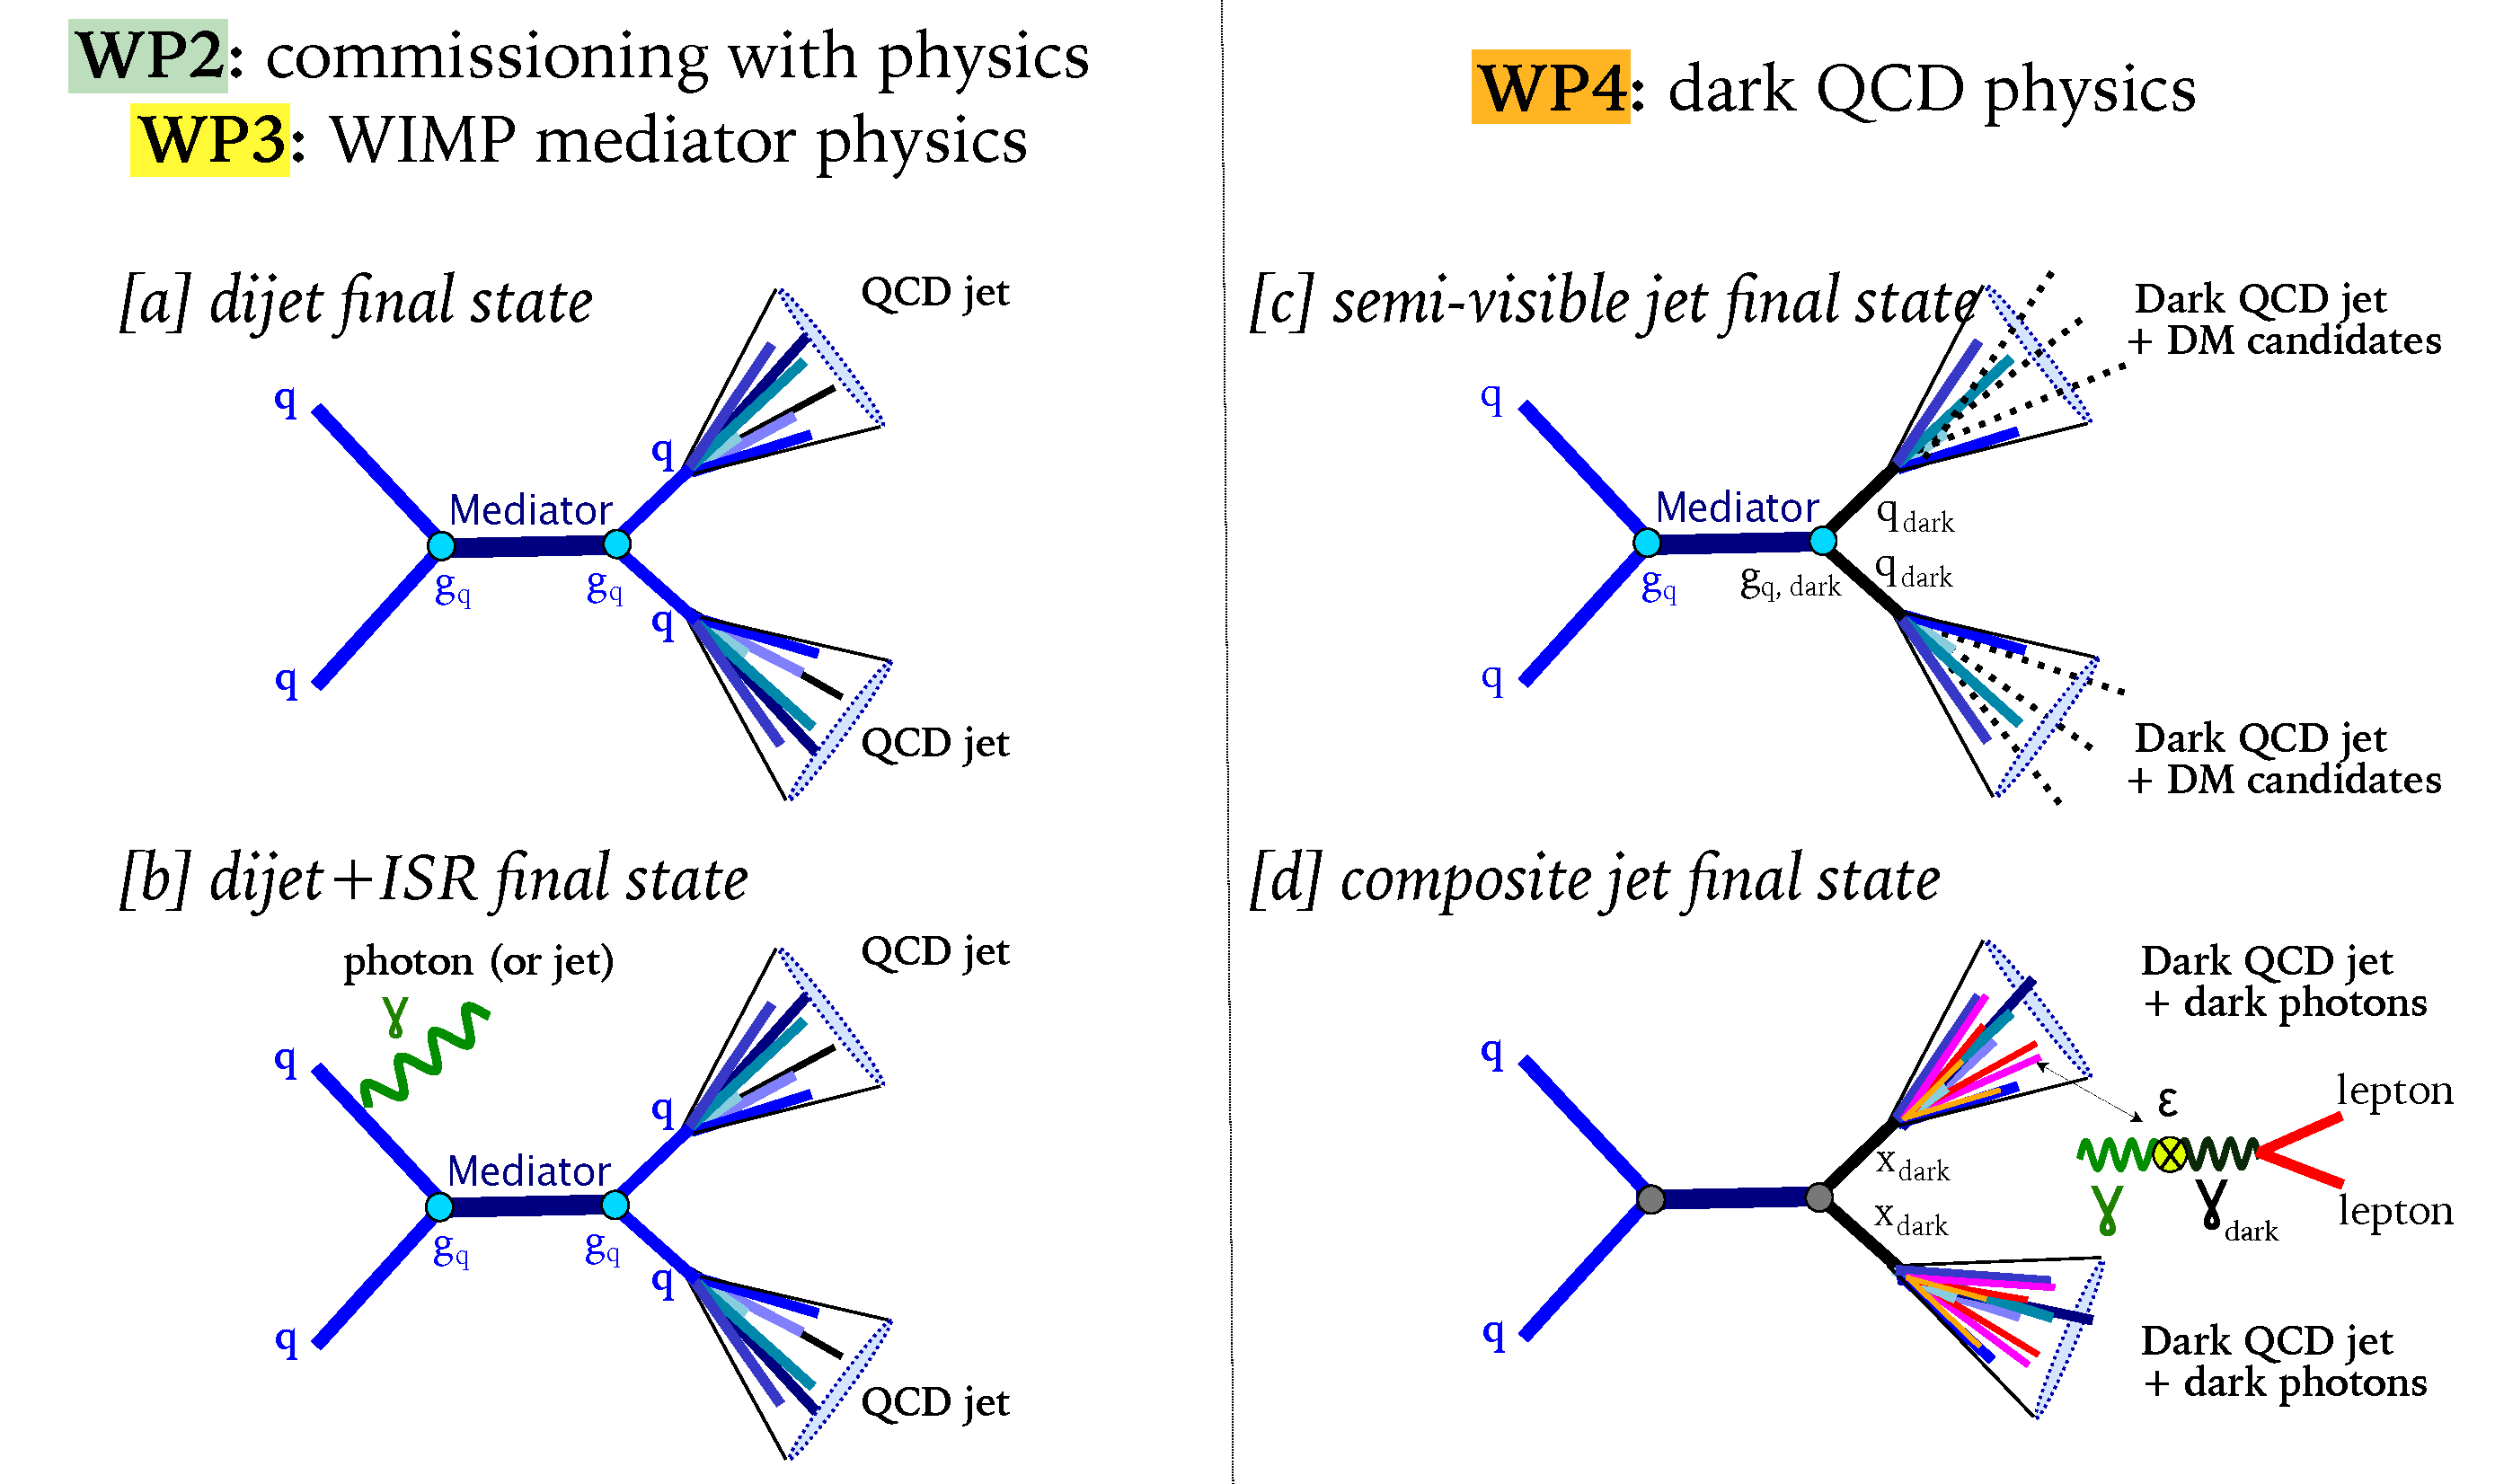
\includegraphics[width=0.65\textwidth]{figs_B2/feynman.pdf}
\caption{Sketches of search signatures in this proposal.\color{black}\label{fig:feynman} }
\vskip2pt
\end{center}
\end{wrapfigure}
%\vskip5pt

Simplified models are well-motivated benchmarks at a time when no experimental hints are observed, as they allow for a systematic exploration of experimental search targets by scanning the parameter space (DM mass $m_{DM}$, mediator spin and mass $m_{Med}$, couplings to DM $g_{DM}$ and SM $g_{SM}$).
Exploration of yet unprobed parameter space for mediator decays as in the left-hand side of Fig.~\ref{fig:feynman} motivates the searches in WP2 and WP3. 

%More to defend simplified models, maybe too much?
%Furthermore, motivating searches for only a handful of new particles with simple interactions even if they are part of a complex spectrum is conceptually supported by how ordinary particles were uncovered in the history of the SM: the first particles discovered were the most common ones, and further complexity was unraveled at a later date. 
%These searches will be used to commission trigger improvements in WP2-3 will improve  much greater sensitivity with respect to previous searches , and employ simplified models as building blocks for more complex theories (WP4). 

%Aims of this paragraph: introduce dark sector models and hidden sector
In parallel to considering WIMP DM models, it is also imperative to \textbf{consider alternative DM models that could have escaped detection} so far. 
An example is a class of models including mediator-like particles that do not directly connect DM and SM, but rather provide a \textbf{hidden portal} with much weaker interactions between a more complex dark sector and SM particles~\cite{Strassler:2006im}. 
\\
\indent
The symmetries of the SM can be used as guiding principle to construct the particle spectrum and the interactions of the new dark sector. 
A \textbf{new U(1) symmetry} introduces a portal particle called \textit{dark photon}~\cite{Holdom:1985ag,Curtin:2014cca}.   
The dark photon mixes with the ordinary photon, leading to rare but observable signatures from its decays to SM particles. 
This model is currently used as a benchmark for many non-LHC experiments and for future facilities~\cite{Strategy:2019vxc}. 
%Why according to Shaposhnikov (who motivated benchmarks): doesn't quite convince me. 
%Light particles have become a more popular search target because they can be used to solve particle physics  
%g-2, only in connection with DM
%and astrophysics anomalies 
%Pamela (bleurgh)
%too-big-to-fail as opposed to WIMPs - self-interactions
Models with a \textbf{new SU(2)}, also termed \textit{dark QCD} models for their similarity with SM QCD, predict that their fundamental components (dark quarks, $q_{dark}$) are confined at an energy scale that can be comparable to that of QCD. 
This leads to signatures of highly collimated particles, resembling hadronic jets that include dark sector particles and their decay products (\textit{dark jets}). 
\\
\indent
A number of concrete realizations of theories including one or more of those new symmetries exist (e.g. asymmetric DM~\cite{Zurek:2013wia}, electroweak SUSY models~\cite{Cheung:2009su}, self-interacting DM~\cite{Tulin:2017ara}, strongly-interacting DM~\cite{Bernreuther:2019pfb}). 
The large number of parameters and particles, and their subsequent variability in terms of experimental manifestations, mandates \textbf{signature-driven searches} rather than searches targeting specific theory benchmarks. 
For this reason, the data-taking techniques in this proposal are designed to \textbf{record data that could contain a variety of these signatures, and that would otherwise be discarded}. The searches in WP4, using the dark jets signatures shown in the right-hand side of Fig.~\ref{fig:feynman} \textbf{target two uncovered dark sector signatures} as concrete use cases for this dataset. As shown in the right-hand side of Fig.~\ref{fig:feynman}, we will first search for dark jets containing thermal relic DM particles (semi-visible jets) produced from the decay of a $Z’$~\cite{Bernreuther:2019pfb,Cohen:2017pzm}, and subsequently for dark jets where the showering process interleaves dark photons and dark hadrons, leading to hadronic jets with an anomalous leptonic content (composite jets)~\cite{Cheung:2009su,Park:2017rfb}.
%Further thoughts are in here
%%Together or individually, mediator particles above and dark photons can also be part of a dark sector set of particles that do not interact significantly with the SM, including the DM candidate~\cite{Felix}. 

%Another possible story (but longer)
%Building blocks: dark QED
%Why attractive
%Conceptual connection to vector mediator above
%Why neglected
%Next-on: dark QCD
%Why attractive
%Why neglected




%For this reason, systematic exploration of these models does not proceed by scanning the theory’s parameter space, but rather by mapping the characteristics of different possible configurations of parameters and ensuring that no experimental stone is left unturned. 
%Searches for this kind of models have recently started taking shape at the LHC, in parallel to a vigorous pursuit by planned and existing non-LHC experiments~\cite{PBC}. 



%DM can't catch light DM even though there are a lot of tries
%So we go after the mediators again

%- Large experimental variability
%- Many motivations for lepton-jet models, but they neglect hadronic dark sector particles (eg SUSY lepton-jets below)
%- So we start where we can, and where we have motivations - B-L? 

%Peter's suggestion for B1, but I don't know where to add it? 
%The only thing I miss and I can understand that it can be hard to fit in is a motivation of WIMPs and
%in particular dark QCD. Could one maybe add just a little a la:
%The nature of dark matter is difficult to understand, because even today there is five times more
%dark matter than normal matter, this is only after essentially all normal matter in the Universe
%annihilated microseconds after the Big Bang (only 1 in 10,000,000,000 protons survived). The WIMP
%solution is a weakly coupled particle that yields the observed DM abundances by being weakly
%produced. It is attractive to search for WIMPs at the LHC because the energy of the accelerator
%allows studies above and below the electroweak phase transition. In Dark QCD one instead assumes that
%the abundances are similar because there also was an annihilation in the dark sector of the Universe
%and so Dark QCD models can potentially also explain the matter-antimatter symmetry observed in the
%Universe. It is attractive to search for Dark QCD at the LHC because it is a QCD collider and so one
%could expect that if there is a coupling between QCD and Dark QCD then we are likely to produce Dark
%QCD mesons and baryons at the LHC.%Check the latter

%SUSY lepton-jets: https://arxiv.org/pdf/0909.0290.pdf
%The cascades to N ̃1 may also result in colored particles and hence QCD-jets, but for the purpose of the current study we will assume that a substantial fraction of such cascades result in no colored particles. This is not a strong assumption as it is satisfied in many concrete examples of MSSM spectra [11], and may even be discarded altogether in actual lepton jet searches including QCD-jets.

%Existing text
%, and as a consequence it is only extremely feebly connected to electrically charged particles - I should probably talk about its decays
%too ambiguous? it decays into fermions as if it were a photon
%rather than direct interactions with


%This is one of the cases in which simplified models are used as building blocks for more complex models.


%In WP4, I will make use of my expertise in the reconstruction of hadronic jets and non-standard data taking technique to search for two classes of theoretically-motivated DM models that include a new strong force within the dark sector (dark QCD), using novel data taking techniques necessary for uncovering their signatures. 
%With these searches, this proposal will contribute to the systematic mapping of the territory of hidden sector signature, in synergy with other LHC and non-LHC searches. 

The emergence of new models for DM and new ways to look for them indicates that the DM community is thriving.  
Depending on the SM-DM interaction strength and on the DM characteristics, a wealth of new experiments can contribute to the quest for WIMP and non-WIMP DM~\cite{Beacham:2019nyx,Bertone:2019irm,Barausse:2020rsu}. 
It is clear that, given the breadth of possible explanations for DM, an equally broad experimental and theoretical approach is needed, 
and that new synergies can be exploited beyond the already-mentioned complementarity between DD/ID and colliders searches. 
This consideration inspires the work planned for WP5, taking place within newly established common platforms for dissemination of results and tools, in the spirit of open and collaborative science. 

\subsection{The state of the art in experimental tools for discovering dark matter and new phenomena}
\label{sub:stateOfTheArtExperiment}

\subsubsection{LHC and ATLAS: overview and schedule}
\smallskip

The LHC will restart operations in Summer 2021 and continue delivering proton-proton collision data until the end of 2024. In this data taking period (called \textit{Run-3}), up to 250/fb will delivered to the ATLAS experiment~\cite{ATLAS2008}.%{JINST2008}. 
It is expected that the bulk of the data will be collected in 2022 onwards, after a first period of commissioning for the machine and the experiments. 

In Run-3, the LHC collision energy will not be significantly increased, and the dataset size will be only slightly larger than the Run-2 dataset (189/fb). 
It is clear that the discovery potential warranted by the upcoming dataset will not improve by statistics alone. 
\textbf{New methods and technical innovations are required to discover rare processes}, at a time when traditional data-taking confirms the SM.%, mandates technical innovation. 
Innovating the ATLAS data acquisition and selection system is an integral part of this proposal, 
as the key to extract a much larger amount of useful information from the upcoming LHC dataset. 
This proposal is especially timely given that the improvements within \textsc{Realdark} can be tested with physics in early data and are required to be made in advance of the LHC production phase for full exploitation of the LHC dataset. 

\subsubsection{The ATLAS trigger and its upgrades}
\smallskip

Recording the entirety of the LHC data (up to 30 million collision events/second) is unfeasible due to storage and computing limitations. 
Therefore, \textbf{only a small fraction of interesting events is selected} by the ATLAS trigger system. 
%The rest are discarded forever. 

The ATLAS trigger is composed of two levels~\cite{ToBeCited}. %2015TriggerPaper
The first hardware level (L1) performs an initial coarse selection within 2.5 $\mu s$. 
Selected events are passed to the software-based High Level Trigger (HLT), implemented on a computing farm. 
The HLT performs a more refined event reconstruction and data analysis \textit{online}. 
This informs the final decision on whether to discard the event or keep the full detector information for further \textit{offline} reconstruction and analysis of electrons, muons, photons, jets, ... (called \textit{physics objects} in the following). 
The total event rate that can be retained after the HLT decision is directly \textbf{limited by the available amount of storage space}. 
%since traditional offline analysis currently requires the full set of detector information for reconstruction of physics objects (e.g. electrons, muons, photons, jets...). 
The rates of useful events recorded for offline analysis are also indirectly limited by the available HLT computing: 
a number of high-level features that would help in distinguishing signal from background are \textbf{too expensive to reconstruct given the available HLT resources}. 
%An example of such a feature is the track-collision vertex association for physics objects, 
%as this enables removing spurious contributions from simultaneous proton-proton collisions other the one of interest (pile-up). 
These limitations impairs the sensitivity of searches where signals are buried in high-rate backgrounds and motivates the improvements in WP1. 

The ATLAS trigger is undergoing significant upgrades for Run-3~\cite{Aad:1602235}. 
The ATLAS L1 trigger will be equipped with new electronic boards that allow for a more granular and efficient first-pass selection. 
As part of my StG, my team has developed control software for the board which will permit using information from the entire hadronic calorimeter at once (gFEX)~\cite{Tang:2016ded}, 
and contributed to the software for the new jet board (jFEX)~\cite{Bauss:2018nde}. 
Furthermore, the HLT software is being rewritten as a multithreaded framework~\cite{Bielski:2674286} and the computing power of the ATLAS HLT farm will increase significantly. 
The combination of optimized algorithms\footnote{See Ref.~\cite{ATL-PHYS-PUB-2019-041} %Elsing 
for an example of the improvements from optimizing tracking algorithms on simulated data containing 200 simultaneous collisions for the ATLAS high luminosity upgrade}. 
and increased HLT capacity will allow a more widespread availability of tracking information at the trigger level with respect to Run-2. 
This information is crucial to reject backgrounds from simultaneous proton-proton interactions (pile-up), which in turn is a limiting factor for the sensitivity of LHC DM searches. 
Moreover, for the first time in ATLAS, it will be possible to write out object reconstructed directly at the HLT in combination with selected raw detector information in regions of interest with a technique called Partial Event Building, or PEB, currently only used for muons calibration and $B-$physics. 
Testing and exploiting these upgrades is an integral part of this proposal. 

%Among those, a full overhaul of the electronic boards that read in calorimeter information is foreseen. 
%The board that reads information from the electromagnetic calorimeters (eFEX) will allow for more refined distinction between electrons and photons already at L1. 
%This motivates the implementation of alternative data-taking techniques to overcome these limitations, as proposed in WP1 and discussed in the next section. 
%This can probably be removed since I don't use it directly anywhere else? 

\subsubsection{Review of analysis strategies for DM and related particles at the LHC}

Traditional searches for \textbf{WIMP Dark Matter} at colliders seek an excesses of imbalanced events where weakly or non-interacting particles escape the detector unseen~\cite{Boveia:2018yeb}. 
If the processes sought in traditional searches via a mediator particle as described in Ref.~\ref{sub:stateOfTheArtTheory}, 
resonant signals should also be present from the decays of the mediator into SM particles.
Searches for visible decays of the mediators are complementary to searches for invisible particles~\cite{CMSSummary,ATLASSummary}  
%Another point to look for visible decays, but not relevant here: 
%Considering the simple picture of \textbf{Fig. X}, invisible signals will be suppressed with respect to visible signals if the DM particle is much heavier than the particle mediating the interaction and invisible decays must occur off-shell. 
%\textbf{Decide: dijet/di-jet}
%Searches for visible signatures is an established complementary alternative to searches for invisible particles, with different challenges and sensitivity~\cite{ToBeCited}.%Summary plots 
Visible mediator decays connect DM mediator searches with the well-known class of searches for new resonances at particle colliders. 
New resonant particles have a large array of theoretical motivations beyond DM, and are not yet fully constrained by existing searches~\cite{Kim:2019rhy}%{Craig2bodyResonances} 
\\
\indent
The searches in WP2 and WP3 in this proposal focus on a well-motivated yet experimentally challenging category of decays (see e.g.~\cite{Chala:2015ama}). 
Having been produced via a quark-quark vertex, the mediator will also decay back into quarks (Fig.~\ref{fig:feynman} [a]). 
The signature of this process is a resonant peak in the two-jet (dijet) invariant mass, peaking atop the smooth QCD background.
%%The relatively low background rates of high-mass hadronically-decaying resonances permit collecting all events in full above a threshold of approximately 1 TeV~\cite{ToBeCited}. 
Below 1 TeV, large amounts of QCD backgrounds overwhelm the experiment’s data storage resources, forcing to discard signal together with background~\cite{ToBeCited}. %high-mass dijets  
For this reason, dijet resonances with masses around the electroweak scale ($\approx$100-200 GeV) have been very difficult to probe with standard data-taking techniques. 
\\
\indent
Discovering \textbf{resonances with sub-TeV masses require novel data taking techniques and/or targeted signatures}. 
%During my StG, my team and I have pursued both directions within ATLAS. 
Following the example of the Data Scouting technique in CMS~\cite{ToBeCited} and the Turbo Stream in LHCb~\cite{ToBeCited}, my StG team and I prototyped the \textbf{Trigger Level Analysis (TLA) technique} for jets. 
In TLA, high-level jet information is retained for all dijet events reconstructed by the HLT, discarding raw data. 
TLA allows for for a much smaller event size and much higher event rates~\cite{ToBeCited}.%TLA PRL 
\\
\indent
In normal-luminosity data-taking conditions, TLA dijet searches are still limited by the L1 event rate to resonances with masses above 450 GeV, 
and other detector signatures with reduced background rates are required to reach lower mediator masses. 
One such signature that my collaborators and I introduced to the LHC in Run-2 is the \textbf{dijet+ISR signature}. 
Here, the resonance recoils against a high-p$_{\rm{T}}$ photon or gluon radiated from the initial-state quarks (Fig.~\ref{fig:feynman}, [b]). 
The requirement of an energetic object at the HLT reduces the background and allows to reach lower mediator masses, 
but limits the signal acceptance. 
Lowering the threshold on the ISR objects would increase the mass coverage and signal acceptance.
This motivates combining the TLA technique for the dijet+ISR signature for the first time in ATLAS\footnote{The CMS search in Ref.~\cite{ToBeCited} %CMS dijet+ISR
combines the dijet+ISR signature with the Scouting technique, but it does not surpass the sensitivity of the offline ATLAS search as it is limited to a limited Run-2 dataset with special triggers.}, as planned for WP3. 
\\
\indent
The combination of ATLAS and CMS low-mass dijet resonance searches (TLA/Scouting and dijet+ISR searches)~\cite{ToBeCited}
including searches targeting resonances decaying in heavy flavor quarks~\cite{ToBeCited} %di-b
and where the resonance is boosted~\cite{ToBeCited} %CMS and ATLAS dijet ISR boosted
improves the sensitivity of LHC experiments but still leaves significant room for discovery around the EW scale. 
This is a region where the weak force mediators reside, and that is favored in WIMP and non-WIMP $Z’$ models fitting ID excesses~\cite{ToBeCited}. %Hooper&Leane  
To date, searches in this region are only sensitive to coupling strengths well above those of the weak force. 
Pushing the collider sensitivity to be comparable to DD in this region will help validate and characterize a possible DM interpretation of these results~\cite{Ellis:2018xal,Kang:2020huh}.

\color{red}\textbf{TODO: References done up to here}\color{black}

\begin{wrapfigure}{R}{0.5\textwidth} 
\begin{center}
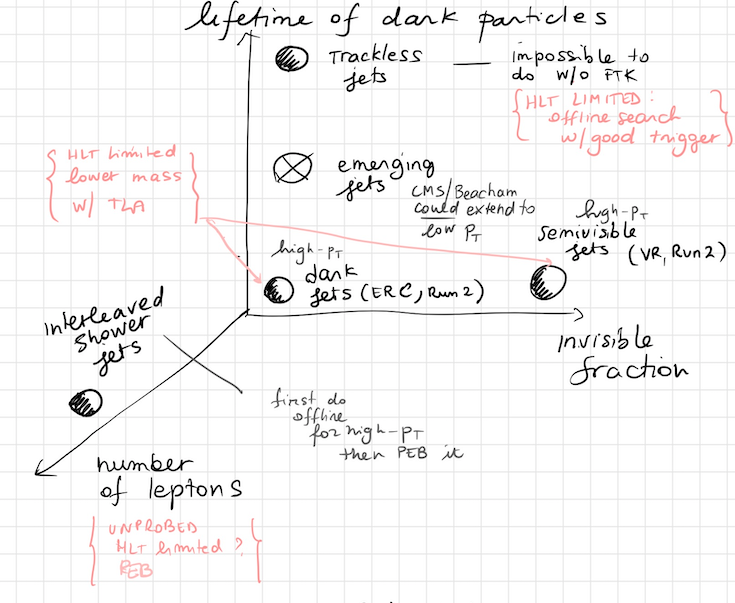
\includegraphics[width=0.5\textwidth]{figs_B2/DarkSectorSketch}
\caption{Sketches of covered and uncovered search signatures for dark jets. \color{red}\textbf{TODO: Add references to picture}\color{black}
\label{fig:darksectorssketch} }
\end{center}
\end{wrapfigure}
\vskip-10pt

%Alternative text because Dark QCD is sometimes strongly interacting?
%Partly motivated by the constraints set on such particles by first-generation direct searches and by results obtained in the first phase of the LHC data taking, the DM community has recently started to generalize the flagship searches for these weakly interacting massive particles (WIMPs) by expanding the search program for particles with either stronger or much weaker interactions with SM particles than what predicted by WIMP theories~\cite{FIMPs, StronglyInteracting}, or much lighter particles~\cite{DarkPhotons, ALPs}, or much more massive objects (e.g. Primordial Black Holes)~\cite{GW paper}~\footnote{Such scenarios can also fit the measurements of the relic density of dark matter through different mechanisms~\cite{FreezeIn}}. 
 
While the landscape of DM mediators is well mapped even though not yet fully constrained, 
the state-of-the-art of \textbf{hidden sector and dark QCD searches} leaves much room for joint experimental and experimental improvement.

Hidden sector models generally imply more difficult detector signatures than more established benchmarks. 
An example are particles with a long lifetime, whose decays away from the interaction point are not suited to standard reconstruction techniques~\cite{ToBeCited}.
Unusual features, such as displaced decays or unexpected particles within the busy environment of a hadronic jet, are too expensive to reconstruct at the HLT and require specific data formats. %DRAW
This forces searches to rely on triggers that let large amounts of background through (e.g. missing transverse energy or purely hadronic triggers) and subsequently induce limitations on the signal rates, or to trigger on specific signatures and partially lose model-independence. 
This motivates the use of the TLA+PEB technique in this proposal, so that more complex features can be reconstructed after only a coarse preselection, limiting the loss of search generality. In TLA+PEB, the event size is reduced with respect to traditional data analysis, so that the signal rates recorded can be increased. 
 % with a small enough event size and increased signal rates with respect to traditional searches.%, limiting the loss of generality of the search. 

The approach for choosing and designing Run-3 searches to be performed using this technique within the timeframe of this proposal is signature-driven rather than model-driven. 
As specified in Sec.~\ref{sub:stateOfTheArtTheory}, we adopt the grounding assumption that the confinement scale is sufficient to produce dark jets. 
 %Ohm Soffer review 
As an initial guide to the experimental state-of-the-art for the searches in WP4, dark jets can be classified according to their main features. 
Extending Ref.~\cite{Cohen:2017pzm, Park:2017rfb}, Fig.~\ref{fig:darksectorssketch} characterizes dark jets according to the following.  

\noindent
\textbf{1.} Depending on how many of the constituents of the the dark jet are long-lived, the dark jet will appear in the detector at different distances with respect to the interaction point. ATLAS and CMS searches pursue these signatures, looking for \textit{emerging}~\cite{Sirunyan:2018njd} or \textit{trackless jets}~\cite{ToBeCited} jets and for the long-lived particles themselves~\cite{ToBeCited}. Together with colleagues from LPSC Grenoble and Witswatersrand, I am pursuing the first-ever LHC search for signatures of jets whose constituents are prompt and fully visible but fragment differently (\textit{prompt dark jets})~\cite{Park:2017rfb}, with a publication expected by Fall 2020. \\
\textbf{2.} The dark jet may be constituted by a sizable fraction of invisible particles, e.g. stable dark sector particles and DM candidates, and appear as a \textit{semi-visible dark jet}. In this case, we assume that the lightest particles in the dark sector are the DM candidates following Refs.~\cite{Cohen:2017pzm,Park:2017rfb,ToBeCited}%Felix
\footnote{Dark sector / dark pion decays into SM particles motivate other searches that will be connected to the ones in this proposal, for example emerging/trackless jets and searches in the review of Ref.~\cite{ToBeCited}}.%Kribs, https://lhcbproject.web.cern.ch/lhcbproject/Publications/LHCbProjectPublic/LHCb-PAPER-2016-065.html
\\
\textbf{3.}  The dark jet may contain an unusual number of leptons, from leptonically-decaying dark photons. In this case, jets composed exclusively of leptons (lepton-jets) are covered by ATLAS and CMS searches~\cite{ToBeCited}.%LeptonJets
%\textbf{This part needs to be sharpened...} 

From this classification, \textbf{Semi-visible jets}  (Fig.~\ref{fig:feynman} [c]) are experimentally uncovered at the time of writing. 
%Should I say this? 
%~\footnote{I am involved in an ongoing search for semi-visible jets in ATLAS and CMS with Run-2 data, but the benchmarks used and mass range are different to those used in this proposal. There is also an ongoing CMS search using Run-2 data.}.
Similarly,  \textbf{composite jets} where dark QCD and dark photon showers are interleaved producing a cascade of leptons and hadrons within the same jet (Fig.~\ref{fig:feynman} [d]) have not been sought at the LHC before. 
This motivates the choice of the two WP4 searches. 

Experimental attention generally stimulates theoretical development and extensions of unprobed models, as well as efforts towards their systematic classification. 
As part of WP5 in this proposal, we will organize workshops and open a number of discussion channels with the theory, astroparticle, non-collider and nuclear physics communities. 
This cross-talk will be useful for input on search targets, on the simulation of benchmark models and for the contextualization of search results.

\color{red}\textbf{TODO: Reorganization done up to here}\color{black}


\subsection{Objectives}
\label{sub:objectives}
\smallskip

The proposal’s overarching aim is to discover or constrain the particle nature of dark matter via its production at the LHC and the contextualization of these results in the global DM theoretical and experimental landscape. 
The basis for reaching this aim is the implementation of data-taking techniques that enable the ATLAS experiment to obtain a much bigger physics output from the upcoming LHC dataset without requiring a significant increase in resources. 
Physics results and software tools resulting this proposal will be shared with the broader DM community. 
As outlined in part B1, this proposal is composed of 5 interconnected work packages. 
The objectives of each WP and their intermediate key goals are described in the following sections. 

% and their interconnections are displayed in \textbf{Fig.~\ref{fig:WPs}}. 

\subsubsection{Objectives of WP1}

The first objective of WP1 is to \textbf{deploy a comprensive TLA stream in ATLAS within the new multithreaded ATLAS HLT software}. %mentioned above?
In Run-3, this project will allow offline-quality photons, muons and electrons to be used for physics analysis, in addition to jets. 
The success of the jet prototype has been demonstrated in Run-2 within my StG. 
The use of a jet TLA allowed to lower the HLT jet threshold from 420 GeV in traditional analysis to 220 GeV in TLA, bringing orders-of-magnitude improvements in the number of recorded events. 
A TLA implementation of HLT photons will bring significant improvements to the sensitivity of the dijet+ISR DM mediator search. 
The HLT analyzes all photon and electron candidates that have a $p_{\rm{T}}$ above 30 GeV, 
while only single-photon events with a $p_{\rm{T}}$ above 150 GeV are retained in traditional analysis. 
The work done and lessons learned in the case of trigger-level jets will be the stepping stone for adding photons to the TLA stream, 
and doubling the signal acceptance for the dijet+ISR search. 
The implementation of electrons and muons in TLA will follow that of photons.
% but they will not be a priority for first data as the difference in thresholds between online and offline events is limited. 
While electron and muon TLAs can still bring significant improvement to e.g. dark photon searches below the Z peak~\cite{ToBeCited}, %CMSDimuon
the aim of this work is to gain confidence with the challenges of reconstruction and calibration of different physics objects with constrained computing resources. 

The second objective of WP1 is to \textbf{implement and reconstruct a data stream combining physics objects reconstructed at the trigger level and selected raw information in restricted regions of the detector}, through the combination of the TLA and Partial Event Building (PEB) techniques. 
Deployed for the first time in ATLAS in this proposal, this combination will maintain a sufficiently small data format with an amount of information equivalent to traditional techniques. 
It will be a necessary ingredient to enable searches in WP4, and can be used for the characterization of any excesses observed in TLA searches. 
%The overall outcome of this work will be a technical publication detailing the early Run-3 trigger.  
Preliminary estimates based on the Run-2 $B-$physics PEB %cite muon paper if available
place the size of TLA+PEB events to less than half of a standard event. 
To remain advantageous, TLA and PEB must have the minimal possible footprint in terms of both storage and computing power. 
Joint work betwen WP1 and WP2-4 will ensure that these constraints are met with dedicated trigger selections and selections.   
The budget of this proposal also includes storage servers that will be used to store this data in 2023-2024. 

As a third objective of WP1, we will \textbf{develop the calibration techniques that are necessary to enable physics analysis} with a reduced HLT-level data format, achieving near-parity with offline performance. 
With my StG team, I have been responsible for reaching a 1-permille agreement between the jet energy scale of HLT jets with respect to offline jets~\cite{ToBeCited}.%TLAPRL 
Within \textsc{Realdark} we will ensure that this is still the case for jets (as our main observables for WP3), as well as for other physics objects. 
\begin{wrapfigure}{L}{0.3\textwidth} 
\begin{center}
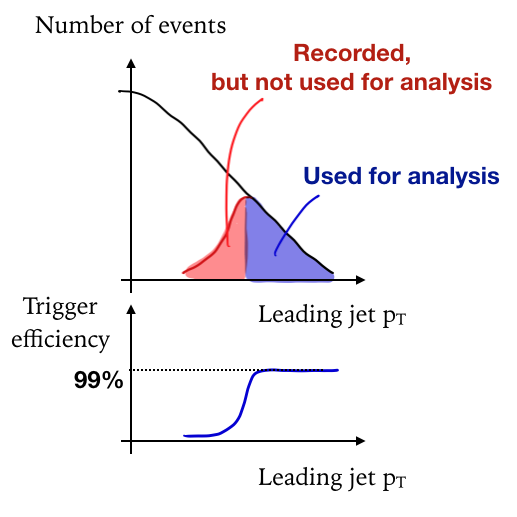
\includegraphics[width=0.28\textwidth]{figs_B2/efficiencySketch}
\caption{\color{black}\label{fig:wastedRate} \small Sketch of how trigger inefficiencies caused by a mismatch between the HLT and offline jet energy scales causes events to be recorded but never used for analysis.} %Trigger operation page
\vskip2pt
\end{center}
\end{wrapfigure}
%\color{red}\textbf{Not sure the following should be here, but it's a good motivation to calibrate HLT objects in case someone isn't convinced. }\color{black} 
Differences in the energy scale of HLT and offline objects also lead to inefficiencies in the trigger selection, as events that should pass the trigger are rejected due to HLT miscalibrations. 
As an example, the minimum $p_{\rm{T}}$ threshold applied to jets used in physics analysis is set to be higher than the HLT threshold due to these differences, leading to a substantial waste in terms of events that are recorded but not used for analysis, as shown in Fig.~\ref{fig:wastedRate}. 
Preliminary studies performed within my StG and with collaborators show that, due to the steeply falling jet energy spectrum, the amount of events that are recorded but never used by offline analysis can be as high as 60\% for certain trigger chains. 
The application of TLA-motivated improved calibration constants at the HLT during e.g. LHC technical stops (allowing sufficient time for the reoptimization of the trigger menu) will improve the fraction of useful data recorded and impact the overall ATLAS data taking strategies. 
%In WP1, my team and I will contribute to the simultaneous derivation of calibration constants for trigger and offline jets. 

The fourth objective of WP1 is to \textbf{further reduce the storage load of TLA events (and more generally ATLAS data and simulation) by compressing this data}. 
TLA data is ideally suited for studies of more aggressive (lossy) compression, since it has already been shown that it can be made robust against loss of information using dedicated calibrations. If compression and decompression algorithms are sufficiently fast (order of milliseconds) they do not significantly increase the amount of resources needed for data processing. 
The use of machine learning techniques for fast and performant compression (e.g. of images) is widespread: inspired by this, my ATLAS collaborators and I have been supervising Lund University Master’s students in preliminary tests to compress TLA data using deep autoencoders~\cite{ToBeCited}. %cite autoencoders paper 
When compressing 2017 TLA jet data, these studies demonstrated that a compression of factor better than 2 can be achieved with a negligible performance loss.  
In this proposal we plan to continue this work and deploy this compression algorithm in a proof-of-principle yet realistic emulation of the trigger system using raw detector data. This is a future-looking study targeting HL-LHC, but if the results are ready to be deployed during the course of Run-3 we will use them for compression of the data recorded with techniques in WP1. 
%Is this also ok with TLA+PEB? 

As the trigger system is crucial for this research program and for the overall ATLAS physics output, the Lund group will maintain a leading role in its operations. 
Throughout the course of this project, the team members will be involved in the development and monitoring of trigger software. 
This is a particularly crucial responsibility during the run up to first data taking, after the complete overhaul of the ATLAS software. 
The Lund group has already taken responsibility roles in the trigger, with the StG postdoc William Kalderon (now a postdoctoral fellow at BNL), who has served for two years as the convenor of the jet trigger and has now moved on to be overall ATLAS trigger menu coordinator. 

\subsubsection{Objectives of WP2}

The overall objective of WP2 is the commissioning of the new trigger techniques using early LHC data, and their validation using well-established physics observables. 
These observables will be used to evaluate the performance of the calibration techniques and take corrective measures if needed, still to be implemented in time for the production phase of the LHC. 

The first focus of WP2 is the \textbf{determination of the performance of HLT jets and photons, and of electrons and muons} at a later date. 
Together with our collaborators in ATLAS, we will evaluate the energy scale and the uncertainty of HLT objects using early data and simulation. 
I am an expert in those topics, having derived the very first iteration of the energy scale uncertainty~\cite{ToBeCited} %Jet cross-section and my thesis 
and having supervised a number of students on this topic since. 
Within my StG, we measured the performance of both offline and trigger jets in early Run-2 data using the same metrics and techniques, 
and we intend to do the same in Run-3 for an impact on all ATLAS early measurements and searches.  

We will use \textbf{early data to commission the new Run-3 trigger software} in the HLT dijet mass spectrum. 
The experience at the beginning of Run-2, where my collaborators and I observed a L1 trigger misconfiguration in early jet data that limited measurements and searches~\cite{Collaboration:2035503}, showed that this is a mandatory validation step to take after upgrades. 
Subsequently, we will repeat this process for PEB muons and electrons, using the dimuon and dielectron mass peaks from the decay of standard candles ($Z$ and $J/\psi$) \textbf{[10]}. 

\begin{wrapfigure}{R}{0.5\textwidth} 
\begin{center}
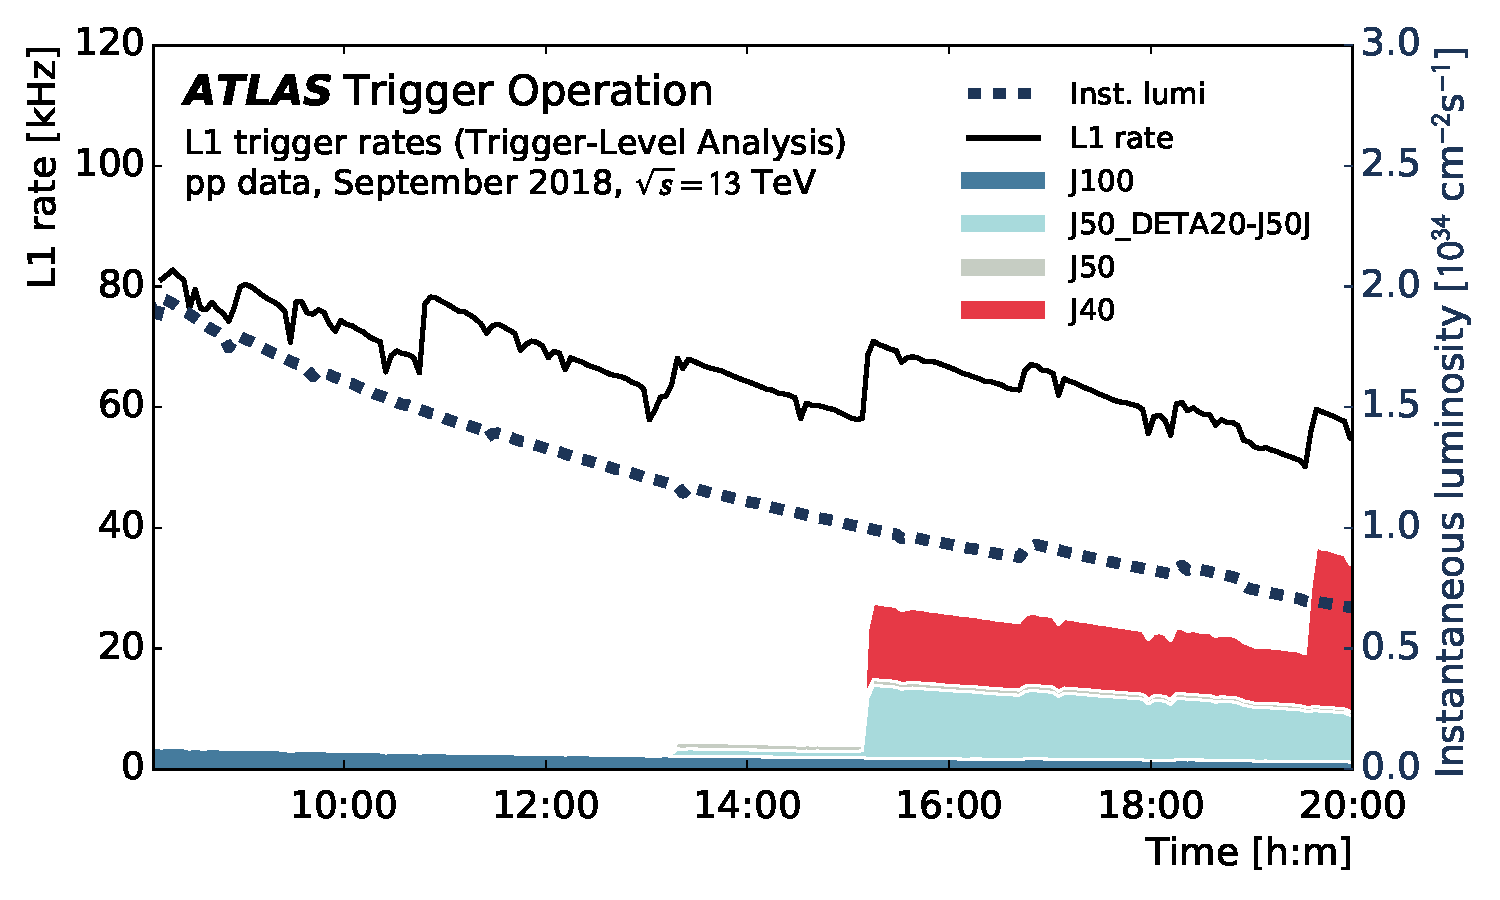
\includegraphics[width=0.48\textwidth]{figs_B2/TLAPublicWinter2019_L1Lumi.pdf}
\caption{\color{black}\label{fig:triggerLowThreshold} \small In Run-2, the underutilization of HLT resources at low LHC instantaneous luminosity allowed my team and collaborators to design TLA L1 triggers with reduced $p_\mathrm{T}$ thresholds~\cite{ToBeCited}.} %Trigger operation page
\vskip2pt
\end{center}
\end{wrapfigure}
%\vskip5pt

If the sensitivity of mediator searches in the dijet mass spectrum improves with respect to Run-2 results, we will publish dijet and dijet+ISR searches using early data.
As an example, if the LHC delivers more than $\approx$ 18/fb of low-luminosity runs, dijet searches can profit from much lower jet trigger thresholds as shown in Fig.~\ref{fig:triggerLowThreshold} and surpass sensitivity with respect to current searches\footnote{The analysis of NN/fb of low-threshold Run-2 data is undergoing as part of my VR project grant, see Funding ID in Part B1}. 

Another important component of this proposal developed in WP2 is \textbf{reproducible end-to-end analysis software for dijet and dijet+ISR DM mediator searches [12]}. 
We will use the RECAST framework to package the entire software stack used for early data analyses so that many of the steps can be executed automatically rather than manually.
Using RECAST at this early stage has three advantages. 
Firstly, it makes intermediate testing and monitoring much faster, as this code can be executed on new data and compared to already-tested data. 
Secondly, it shortens the time required to go from calibrated data to final plots and analysis results in the analysis iteration with the full LHC dataset in WP3.
Thirdly, it can be used as back-end to the REANA framework~\cite{ToBeCited}. %REANA
so that theorists and members of the DM community can test their own signals, as discussed in WP5.  

\subsubsection{Objectives of WP3}

The overall objective of WP3 is to use Run-3 LHC data recorded with the TLA technique to search for new resonances in the dijet mass spectrum, motivated by DM mediators.
In this proposal we will focus on the decays of the mediators to light quarks, but the work in WP1 also enables dedicated searches for mediators decaying preferentially to heavy quarks. 

The main innovation in this WP is the \textbf{dijet+ISR photon search using the TLA technique}, alongside the gluon ISR signature. 
The two channels are complementary: the jet ISR channel is more sensitive due to higher signal rates, but selecting events using photon ISR can reach lower mediator masses. 
Both channels will be much more sensitive than current Run-2 traditional searches, since the threshold on the associated object is lowered from $\approx$ 400 GeV to $\approx$ 220 GeV and from $\approx$ 150 GeV to $\approx$ 40 GeV for jet and photon cases respectively.  
In turn, this increases the signal acceptance of more than one order of magnitude for a mediator mass of 250 GeV~\footnote{The background also increases, but since it is estimated using data-driven techniques as explained in~\ref{sec:methodologies} its increase can be managed without a significant loss in sensitivity.}, 
and it lowers the minimum mediator mass to which these searches are sensitive, as shown e.g. in Ref.~\ref{ToBeCited}.%CMS ISR TLA 
We will also maintain our involvement in the \textbf{full Run-2 + Run-3 dataset dijet TLA} towards a legacy TLA publication covering both LHC runs.

\subsubsection{Objectives of WP4}

%CD: I have the feeling this is a combination of objectives and methods
The objective of WP4 is to use Run-3 LHC data recorded with the TLA+PEB technique for dark QCD searches. 
The most promising parameter space to target will be determined by discussing the theory and broader DM community (WP5), and by using jet measurements to constrain dark QCD phenomenology. 
The rejection of QCD background at the HLT will be crucial for these searches, as it will allow recording higher signal rates in TLA+PEB events. 
The \textbf{search for semi-visible jets} will be performed first, adapting calibration and performance studies in WP1 and WP2 and analysis techniques in WP3 to this signature. 
Subsequently, we will augment the standard reconstruction techniques in WP2 to correctly identify anomalous content (e.g. leptons in jets) needed for the \textbf{composite jet search}.
An additional advantage of the PEB+TLA data stream selected for these searches is that it enables searches for a wide variety of non-standard jet topologies (e.g. photon-jets~\cite{ToBeCited}, %PhotonJets
jets containing long-lived particles~\cite{ToBeCited}) %Long lived jets
at a later date. 
This will have an impact especially after the end of this proposal when the long LHC shutdown is foreseen before HL-LHC and data already taken will be analyzed in further detail. 

\subsubsection{Objectives of WP5}

The overall objective of WP5 is to connect the results in this proposal to the broader experimental community, with a focus on the search for DM, to maximize their impact. 
This WP naturally includes the contextualization, communication and dissemination of results, in terms of tools that can enhance the physics potential of experiments and of DM discoveries or constraints. WP5 also covers my work within synergistic initiatives involving LHC experiments and the broader DM search communities that directly benefit the objectives of WP3 and WP4, started with the Dark Matter Forum and in the context of the update of the European Strategy of Particle Physics. Collectively furthering the DM community’s understanding of the theoretical and experimental landscape for WIMP and dark QCD models will sharpen the LHC search targets. WP5 spans the entire course of this project, and has four goals. 

Firstly, we will collaborate with theory experts in Lund, Heidelberg and worldwide to \textbf{identify the most promising parameter space for the searches in WP4}, in order to develop trigger chains that can best target it~\textbf{[18]}. 
Concretely, this will take place through shared supervision of PhD students and dedicated workshops in Lund, similar to the 2019 Dark Jets workshop~\cite{ToBeCited}. %DarkDijetsWorkshop
These workshops will allow cross-talk with the community interested in comparing and contrasting regular and dark QCD, leading to concrete improvements for MC generation. 

Secondly, I will \textbf{continue co-organizing the Initiative for DM in Europe and beyond (\href{https://indico.cern.ch/e/iDMEu/}{iDMEu})}, a cross-community effort focused on DM that includes the nuclear physics, astroparticle physics and particle physics. 
This initiative has more than 200 endorsers at the time of writing, and will have its first kick-off meeting in early Summer 2020. 
It has the ambition of becoming a permanent forum so that all different communities can identify opportunities to work together and exploit synergies and complementarities. 
Practical outcomes of work within this initiative are summary plots with commonly used benchmarks that enhance the complementarity of the LHC results in WP3 and WP4 with other experiments and astrophysical observations~\textbf{[19]}. iDMEu also includes a component of communication to the general public, also part of WP5~\textbf{[20]}. 

Thirdly, we will \textbf{disseminate the technical outcomes of WP1 to other experiments at the LHC and beyond}. 
This will be achieved via technical peer-reviewed papers that include links to prototype open source software implementations as auxiliary materials and presentation in conferences. 
I have recently become part of the coordination team of the cross-experiment \href{https://hepsoftwarefoundation.org}{HEP Software Foundation} (HSF). 
With its goal of helping experiments meeting the challenges posed by new experimental programmes for HL-LHC, the HSF is an ideal platform to connect the solutions in this proposal to experimental needs~\textbf{[21]}. 
%This goal also includes concrete work on data compression with the EGO/Virgo experiment. 

The fourth goal of WP5 is to \textbf{make results and data from WP3 and WP4 as accessible as possible}, both inside and outside the ATLAS collaboration. 
We will publish the final analysis likelihoods from WP2-4 and implement the end-to-end RECAST analyses in the REANA hub~\cite{ToBeCited}, %REANA
so that they can be scrutinized and reproduced without a need to directly access ATLAS data (which will only be available in open format at a later date)~\textbf{[22]}.
These analyses will become part of a broader effort the cross-experiment \textit{Virtual DM environment} for end-to-end data analysis within the European Science Cluster of Astronomy and Particle Physics ESFRI research infrastructure (ESCAPE), which I will start leading at the beginning of 2020. 
All software implementations within this project will become part of the \href{https://projectescape.eu/services/escape-software-data-catalogue}{ESCAPE Software Catalogue}. 






%As summarised in Part~B1 the proposal is organised into five coherent work packages which logically build using common methodologies to a precision search for new physics with beauty to charm decays. The work packages' main objectives are to: 
%\begin{description}
%		\item [WP1:] Develop new trigger algorithms beyond the standard paradigm of the \LHCb upgrade. This WP builds on the work that the PI has led as HLT Project Leader in the run up to the data taking in 2021, and it is the first use of a revolutionary implementation of a fully software trigger at a collider experiment.
%        \item [WP2:] Perform the first measurements of beauty hadron production cross-sections using decays without leptons. This WP will simultaneously produce measurements that have never been performed and serves as a necessary validation of the trigger system in WP1. In addition, trigger selections to be used in WP5 will be developed. 
%        \item [WP3:] Make precise determinations of the SM predictions for the NP-sensitive \CP observables $\phi_s$ and $\sin(2\beta)$ in \HepProcess{\PB\to\PD\PD} decays. This WP includes measurements using both Run~2 and Run~3 data in order to maximise efficient use of time and resources. It will exploit the new trigger paradigm delivered in WP1 and extend the selections delivered in  WP2. 
%        \item [WP4:] Make the world's most precise determinations of $\phi_s$ and $\sin(2\beta)$ in \HepProcess{\PBs\to\PDsplus\PDsminus} and \HepProcess{\PBzero\to\PDplus\PDminus} decays, respectively, and through comparison to the determinations of WP3 provide a clean NP search. 
%        \item [WP5:] Uncover the structure of the NP measured in WP4 by making the worlds most precise decay-time-dependent determinations of $\gamma$ in \HepProcess{\PBs\to\PDs\PK} and \HepProcess{\PBzero\to\PD\Ppi}. 
%       \end{description}
%The objectives are described in detail in the following subsections.

\section{Methodology}
%\smallskip

The work within \textsc{Realdark} builds novel data acquisition and selection tools and techniques in WP1 and applies them to obtain the physics results in WP2-4. This modus operandi follows my proven track record of bringing challenging improvements to the data-taking system and to the combined performance of the entire experiment, then successfully exploiting them for world-best physics measurements and searches. 
Sec.~\ref{subsub:TriggerRecoSoftware} and Sec.~\ref{sub:CommonMethodsAnalysisTools} describe the methodologies required for reaching the objectives of the WPs described in Sec.~\ref{sub:objectives}. 
Their description follows logically the procedures designed to record, treat and analyze large amounts of raw data towards the dissemination of results that can shed light on the particle nature of DM. %Specific methodologies are described in Sec.~\ref{sub:SpecificMethodsCompression}. 
The project planning is described in Sec.~\ref{sec:ProjectPlanning}.  

\subsection{Methodologies: From LHC collisions to physics objects for analysis}
\label{subsub:TriggerRecoSoftware}

%Should I have "my expertise" here or in project planning? For now, here. 
This section outlines the methods used to record data with the techniques proposed 
and transform these data into observables for the searches in WP2-4. 

\textbf{From LHC collisions to storage} The ATLAS core software infrastructure receives raw trigger and detector information from collisions and assembles it into different data streams. 
Full events that pass the trigger selections are placed in the main data stream for subsequent reconstruction, while partially-built detector data (including TLA and TLA+PEB objects) are placed in specific data streams. 
In WP1, starting from my expertise as one of the main authors of the TLA framework in Run-2, the team will deploy new multithreaded software algorithms that can record jets, photons, muons and electrons, as well as user-defined partial detector information. 
These algorithms are executed if an event is selected by a given L1+HLT trigger ``\textit{seed}'' chain. 
%, in order to reduce the storage and CPU cost of downstream HLT algorithms. 
Given that a large part of the searches in this project occurs at the HLT, a resource constrained environment, an important part of the work occurs prior to data-taking to optimize the CPU and storage resources needed using tools in Ref.~\cite{Martin:2229583} for each of the planned data streams % CostMonitoring talk by Tim 
and determine the optimal stream content and seed chains for the searches in WP2-4. 

\textbf{Reconstruction} Full events are passed through the ATLAS reconstruction software, so that raw detector data can be reconstructed into final physics objects (muons, electrons, jets...). 
While TLA events are already reconstructed within the HLT using inputs and algorithms that are as close as possible to offline~\cite{Aaboud:2017aca,PERF-2017-01,EGAM-2018-01,EGAM-2018-01,Aad:2016jkr}, 
TLA+PEB events will require adapting the reconstruction algorithms to cope with partial detector data as input. 
We can take advantage of trigger-level reconstruction algorithms, where regional reconstruction has already been used to optimize HLT resources~\cite{Aaboud:2016leb}, %Partial event building
and extend existing reconstruction and identification techniques to non-isolated muons and electrons in hadronic environments~\cite{Chatterjee:2019brg,Aaboud:2019wfg}. %Muons in b-jets, heavy neutrinos, and Tuhin Roy's paper

\textbf{Object identification and calibration} Accurate object identification and calibration is crucial to the use of HLT and custom objects for physics analysis.
%I am an expert of jet calibration 
%In the case of TLA, these can be improved at a later date using dedicated algorithms and more refined corrections that are not applied at the HLT. 
Within my StG, I demonstrated a precise calibration is achievable for HLT jets.
Here, we will follow similar approaches for the other HLT objects, keeping the procedures to identify and calibrate HLT objects as close as possible to those for offline objects, with additional data-derived corrections and scale-factors covering the remaining differences. 
%Tracking: where do we need it? Jets, mostly.
A major improvement in the Run-3 calibration procedures is the addition of widely-available tracking information computed by the HLT software, as described in Sec.~\ref{sub:stateOfTheArtExperiment}. 
This allows for improvements in both jet reconstruction and calibration, as \textit{particle flow}~\cite{Aaboud:2017aca} %cite: PFlow
jets combining calorimeter and tracking information can be used at the trigger level, and the same track-based correction steps can be applied to HLT and offline jets~\cite{Aaboud:2018fzt,PERF-2014-03,PERF-2016-04}. %GSC, pile-up suppression
More extensive use of tracks for HLT photons, electrons and muons will be investigated in WP1.   
For example, preliminary studies that I supervised~\cite{8956089} %Leo thesis 
show that the HLT photon calibration in Run-2 was already sufficient for the searches in WP3~\footnote{We expect the situation to improve in Run-3, especially since the preliminary studies did not subtract any of the QCD background, which can be removed using a combination of calorimeter variables (e.g. as in~\cite{STDM-2010-08}).}, but these must be incorporated in the TLA algorithms, and
more thorough use of tracking information could improve the rejection of fake photons and facilitate identification and correct calibration for converted photons in TLA.  
We expect a similar situation in Run-3 for photons and electrons alike, given that the HLT ATLAS electron and photon group plans to align reconstruction, identification and calibration as much as possible, and that residual differences (e.g. from different online/offline calorimeter corrections) can be covered with data-derived factors e.g. from analysis of $Z\rightarrow ee (\gamma)$ events~\cite{EGAM-2018-01}.  
Identification and calibration of HLT muons will also rely on the offline procedures~\cite{PERF-2015-10} %muon performance paper
and additional corrections from $Z$ and $J/\psi \rightarrow \mu\mu$ events. 

\textbf{Performance evaluation} Once the reconstruction and calibration algorithms are in place, their performance needs to be evaluated in data.
We will test HLT objects against well-measured references (offline objects in data and simulated objects without detector effects), according to quantitative figures of merit such as response and resolution, tested against well-measured references. 
In WP2, we will prepare a comprehensive software toolkit for automated, quantitative comparisons between physics objects reconstructed in TLA, TLA+PEB and offline. 
This toolkit will be deployed online, so that HLT problems can be caught as early as possible.
The toolkit will also be used offline to determine the performance of HLT objects.  
The extent to which a mismatch between tested object and reference objects requires intervention (e.g. modification of the reconstruction software, re-derivation of calibration constants...) will be estimated case by case for the WP3 and WP4 searches within sensitivity studies. 
 
\subsection{Common methodologies: analysis and interpretation tools}
\label{sub:CommonMethodsAnalysisTools}

This section outlines the data analysis and reinterpretation methods that are common to the searches in WP2-4, mentioning specific details for each of the searches. 

\textbf{Sensitivity studies} Prior to starting any of the physics analyses in WP2-4, studies are needed to determine the sensitivity of the analysis and refine the parameter space to be targeted (e.g. for producing simulated signal grids). 
These studies are initially implemented as a simplified version of the analysis using events generated for signal and background~\cite{Alwall:2014hca,Sjostrand:2014zea}.   Trigger, detector and calibration effects are implemented using parameterizations and employ full simulation at a later stage. 
For the implementation of the analyses in this project, we will use the RIVET software~\cite{Buckley:2010ar}%RIVET 
as a starting point to analyze generator-level signal and background simulation. 
The advantage of using RIVET is that it easily interfaces with the CONTUR software~\cite{Butterworth:2019wnt}%CONTUR
permitting the use of a large number of LHC measurements to constrain new phenomena. 
This is particularly crucial for the searches in WP4, since measurements of jet fragmentation can already constrain dark QCD showering parameters. 
Sensitivity studies also provide a first testing ground for analysis techniques prior to data-taking, and can be used during the data processing stage 
to understand the level of precision needed for HLT objects in order to be sensitive to certain kinds of signals. 

\textbf{Background reduction and estimate}
Standard Model backgrounds to all searches in WP2-WP4 need to be reduced and estimated. \\
\noindent
The background reduction techniques employed for the searches in WP2-4 select events based on one or more variables that discriminate signal from background.
%These selections will be initially determined in simulation samples, and verified in “validation regions” with limited amounts of signal contamination. 
Simplicity is a driving factor in the choice of background reduction techniques in this project. 
Simpler selections allow searches to remain relatively agnostic to the specific model details, and ease the reinterpretation of results.
% using models others than the ones we employed, enabling the dissemination objectives in WP5. 
In the searches in WP2 and WP3, we will use the angular distribution of the jets as a discriminant between s-channel processes over the QCD backgrounds. 
In the semi-visible and composite jets searches in WP4, we will apply loose selections to reduce the QCD background already at the HLT. 
We will investigate the use and CPU cost of particle flow jet properties~\cite{Aaboud:2017aca}, %PFlow in ATLAS
event shape variables~\cite{STDM-2011-33}, %event shapes in ATLAS
jet substructure techniques and variables~\cite{Larkoski:2017jix}, %Nachman/Moult review, but also ttbar rejection
as well as new dedicated theoretical and phenomenological metrics for measuring QCD jet showering and identifying deviations~\cite{Dreyer:2018nbf,Komiske:2019fks}. %Lund plane, Thaler distance
To complement this \textit{cut-based} approach and to further increase the generality of the searches in WP4, exploratory studies will be performed in the direction of detecting anomalies over the known QCD background using ML techniques (see e.g.~\cite{Cerri:2018anq,DAgnolo:2019vbw,Collins:2019jip}). % employing the same tools as for data compression in WP1. 
This will benefit from the work done within my VR Project Grant, which focuses on unsupervised search strategies specifically targeting resonance searches.
\\
\noindent
%The estimation of the backgrounds, first tested in simulated data, will be derived directly from data wherever possible. 
The background of the dijet and dijet+ISR TLA searches in WP2 and WP3 will be derived directly from data, since the enormous number of events collected excludes the possibility of generating and simulating an equivalent amount, and because QCD simulations are subject to large theoretical and modeling uncertainties.  
For the semi-visible and lepton-in-jets searches in WP4, we will use a combination of data-derived and simulation-driven backgrounds, depending on whether the backgrounds are mainly from QCD (e.g. fake leptons, jets containing heavy flavor quarks decaying leptonically) or from QED and weak interactions (e.g. Z/W+jets where the vector boson decays into leptons and neutrinos, boosted top quarks containing a lepton from the W decay). 
Three background estimation methods are foreseen for the searches in this project: 
\begin{itemize}
\item For searches in WP2 and WP3 we will estimate the smoothly falling QCD background with a functional form or with a continuous parameterization that does not accommodate narrow local excesses such as those from a new resonant particle. The experience gained with the high-statistics Run-2 dijet TLA search within my StG will be crucial to choose the appropriate method among a number of available techniques~\cite{Frate:2017mai,Aaboud:2018fzt,Edgar:2018irz}. %GaussianProcesses,FitMethod
\item For searches in WP4, we will use the ABCD method (e.g. Ref.~\cite{Choi:2019mip,Aaboud:2018lpl}) %ABCD
to estimate the background events in the signal region from normalization and control regions that have a minimal background contamination, defined in terms of independent variables. 
\item For the smaller W/Z backgrounds in the WP4 searches, we will make use of MC simulation using normalization factors derived from control regions in data. 
\end{itemize}
The robustness of the background estimation techniques will be evaluated in partial data scaled to the full expected dataset, using signal injection studies. 

%\textbf{Cross-checks of performance within the analysis selection} The performance of the physics objects in the search will be monitored using the WP2 toolkit, after applying the background reduction selection. 

\subsubsection{Statistical analysis} Analyses in this project will be \textit{blinded}, meaning that the region of phase space or the distribution where a signal is expected is not analysed until the full analysis strategy has been verified from data. We will use control regions and limited amounts of data where a signal would not have a significant impact to disentangle performance issues. 
Before unblinding the signal region, we will finalize background estimation, systematic uncertainties and expected limits. 
% satisfactorily, according to an internal peer-review committee. 
Once this is done, a statistical test will be employed to compare the observed data and estimated background. In this phase, we will also incorporate the systematic uncertainties from the reconstruction and calibration and on the background estimation techniques. 
Given the data-driven nature of the background estimation employed, the systematic uncertainties will mostly impact the signal yields and therefore have a limited impact on the search sensitivity. 
The statistical compatibility of background and data can then be extracted from either the CLs technique~\cite{Read:2002hq}, %CL, from ERC StG
and from tests designed to look for a resonant peak or for an excess in the tails of the distribution~\cite{Choudalakis:2011qn,Aaltonen:2008vt}. %Bumphunter/Tailhunter from ERC StG
We will use a statistical toolkit that enables sharing the final likelihood function, e.g. \texttt{pyhf}~\cite{pyhf}. %pyhf

\subsubsection{Interpretation and dissemination of results} The outcome of the statistical analysis will be either compatibility between the data and the background estimation, or an excess above the background. In both cases, the implementation of the analysis code will be available via RIVET~\cite{Buckley:2010ar}, RECAST~\cite{Schuy:2019awp} and executable on-demand on the \href{http://reanahub.io}{REANA} platform.  
and within the \href{https://projectescape.eu/services/open-source-scientific-software-and-service-repository}{ESCAPE software repository}, 
and the digitized results will be made available on HEPData~\cite{Maguire:2017ypu}. %Rivet
%Note: check that REANA is described somewhere beforehand

\textit{Null result:} The compatibility of data and background indicates that no new phenomena are found within the dataset used for the search. 
Therefore, constraints can be set on benchmark models in the limit setting phase. 
Frequentist or Bayesian techniques~\cite{Cowan:2013pha,Caldwell_2009} %BAT
can be used to set limits on the maximum allowed cross-section of the benchmark process versus the model parameters, e.g. the mass of new resonances.
To extend the results of these searches to any resonant particle, we will also set limits on generic Gaussian-shaped resonances of different widths.
% as done in all searches in my StG, and a responsibility of one of the students for the Run-2 dijet+ISR search~\cite{ToBeCited}. %dijet+ISR 
The outcomes of these searches will be plotted alongside results of other LHC searches and non-LHC experiments within a common theoretical framework. 
For WIMP searches, this will initially follow the methodology of Ref.~\cite{Aaboud:2018fzt}, %DMWG invisible/visible searches
and will evolve following input from the broader community (e.g. from dedicated discussion within workshops and iDMEU). 

\textit{Discovery:} If an excess above the background prediction is observed, it will need to be characterized. 
Following the procedure for blind analyses, the observation will be made public as soon as the excess has been reviewed by the entire ATLAS Collaboration. 
It will be cross-correlated with other ATLAS searches which might see hints of the same process in different final states. 
Identifying the source of the excess and the nature of the resonance (e.g. Refs.~\cite{Khosa:2019kxd,Chivukula:2014pma}) %Vignaroli / Sanz
will become an outmost priority for the team~\footnote{This may lead to changes in the work sharing of this project, as the entire team will be working first-hand with the tools and datasets employed up to that point for a result that has a world-wide impact on the field.} and for the Collaboration. 
In this case, the results of astrophysics and non-LHC experiments will be crucial to ascertain whether these results can be attributed to processes involving DM.

%This needs a study
%An example of a planned step in this direction is the possibility to change in the baseline choice of the main L1 trigger seeding jet TLAs from Run-2. 
%In Run-2, the TLA stream contained all events where there was at least one jet above a certain transverse momentum threshold at L1. 
%The Run-3 TLA stream will contain events where the selection is made on the sum of the transverse momentum of the jets in the event.
%This choice leads to a similar rate as the Run-2 one, thanks to the planned hardware improvements in the L1 trigger, but allows more flexible searches 

\subsubsection{Specific methodologies for WP1: data compression}

Compressing data can lead to further gains in terms of reducing the storage requirements of TLA and TLA+PEB. 
For this reason, this project investigates using deep autoencoders for lossy data compression, in a forward-looking study targeting HL-LHC. 
%Preliminary studies by a Lund engineering (LTH) student that I co-supervised have shown that compressing data using deep autoencoders could lead to large space savings for TLA data and ATLAS data and simulation as a whole, leading to compression factors of 2 with negligible performance loss in TLA data~\cite{ToBeCited}. %Eric's thesis 
The advantage of autoencoders over methods such as Principal Component Analysis is that they are able to learn non-linear correlations among the data, 
and that, once the network is trained, the compression is fast (order 2-5 $\mu s$).
This makes them good candidates to be used in the HLT (latency $\approx$ 300 $\mu$ s). 
Over the course of this project, we will bring the preliminary studies done by the Lund Master's student to a realistic proof-of-principle, within a number of Master's projects and summer projects. 
%Firstly, we will test whether the compression data is compatible with .
%Secondly, we will understand the interplay. 
%Thirdly,   
%investigate compressing raw data. 
%Finally, we will 

%Autoencoders are neural network that implement an approximation to the identity $f(x) \approx x$ using hidden layers with a smaller dimensionality with respect to input and output layers. 
%The smallest-dimensionality hidden layer contains a compressed representation of of the original information. 
%This compressed representation can then be saved to storage instead of the original data format, along with the network implementing the identity. 
%A figure of merit of the fidelity of this identity is the “reconstruction error”. 
%Autoencoders are widely used as anomaly detection algorithms. They are first trained on large amounts of non-anomalous reference data, and then presented with new data. If the new data does not match the reference data, the reconstruction error will be large and can be used as figure of merit to spot anomalies. 



\subsection{Project planning}
%\smallskip

\begin{figure}[!htpb] 
\begin{center}
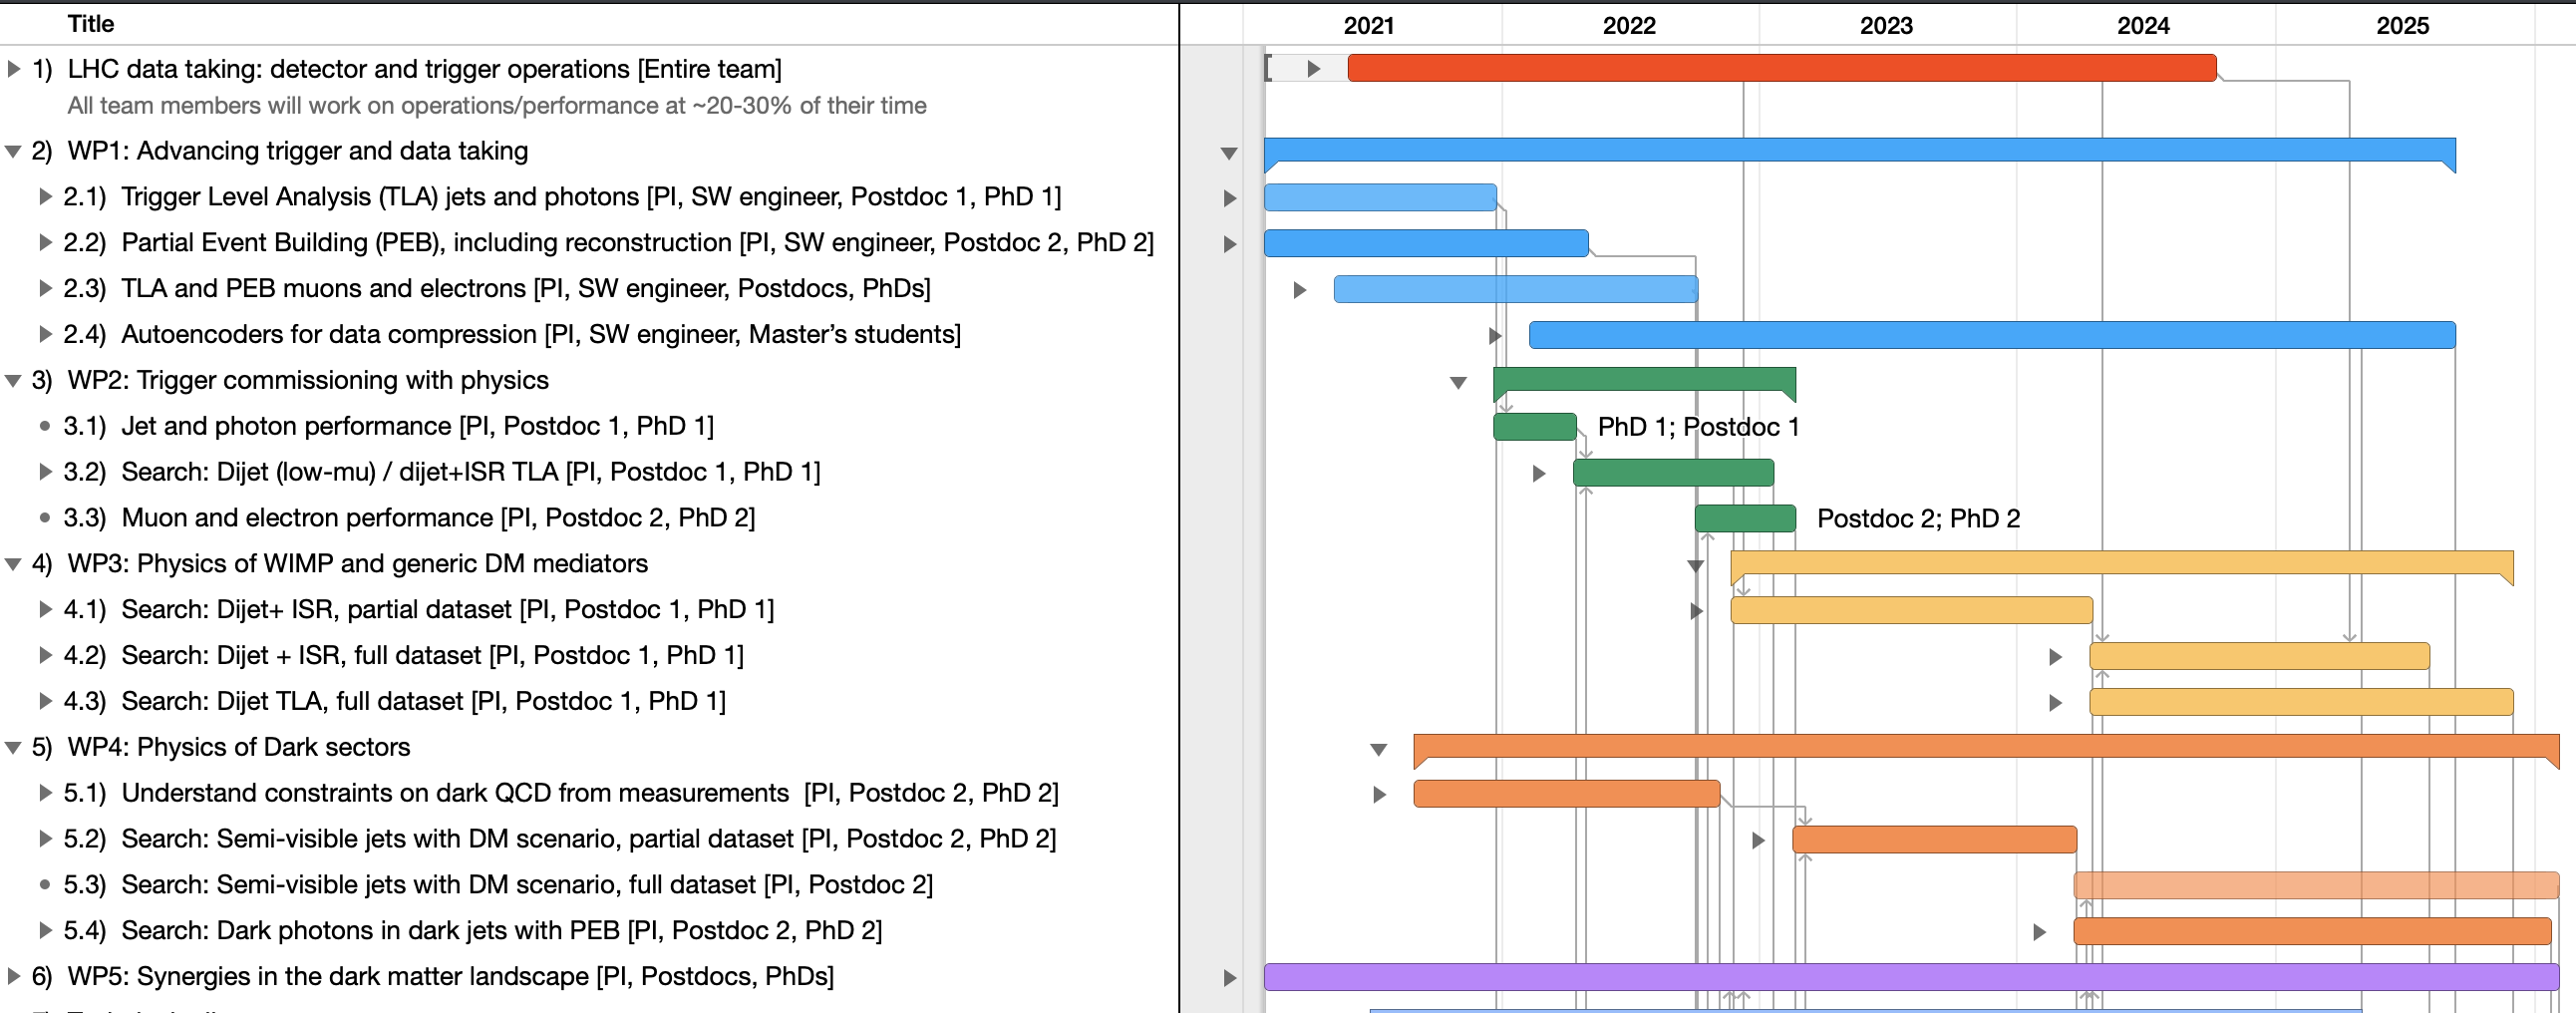
\includegraphics[width=\textwidth]{figs_B2/gantt}
\caption{\color{black}\label{fig:gantt} \small Sketch of project planning and division of work across team members.} 
\vskip2pt
\end{center}
\end{figure}
%\vskip5pt

The research team of \textsc{Realdark} that I will lead as a PI is composed by two postdoctoral researchers, two PhD students and one software engineer.
%Shift this to Resources
The postdoctoral researchers (PD1 and PD2) will be employed for the entirety of the project. 
The PhD students (PhD1 and PhD2) will work within \textsc{Realdark} for their 4-year thesis period. 
Each of the postdocs will work with one of the PhD students on the two physics objectives of WP3 and WP4 respectively, and related technical and commissioning tasks in WP1 and WP2. 
As PI, I will oversee all tasks in the project with day-to-day supervision and regular meetings, and have a hands-on involvement in more complex tasks as specified below. 
%allowing an effective sharing of supervision tasks. 
The software engineer will have a two-year contract at the beginning of the project to ensure the feasibility of the more software-intensive tasks in WP1. 
%end of shift to resources
Fig.~\ref{fig:gantt} provides a project planning schedule, including the breakdown of the work between the team members and intermediate milestones and deliverables marked with \textbf{[N]}. 
It has been prepared using the OmniPlan software~\cite{omni:plan},%Omniplan 
taking into account the interdependencies between the WPs and 
scheduling the work allocation in a way that ensures the feasibility of this ambitious project without overcommitting the team members. 

\subsection{WP1: Real-time analysis and data compression in ATLAS}

%The software implementation of TLA and TLA+PEB techniques and the calibration of physics objects recorded using these techniques represents a significant portion of the work in WP1. 
\textbf{TLA software implementation and calibration of trigger objects} As a preliminary input to this proposal, I have started working on a new Run-3 multithreaded HLT software algorithm that selects and writes out partially-built physics objects in the TLA stream. 
This algorithm will be more flexible than its Run-2 counterpart, and can handle any physics objects. 
By the start of this proposal, we expect to obtain preliminary results of the use of this algorithm on TLA jets. 
In 2021, PI, PD1, PhD1 and the software engineer
will work on the readiness of the core software for photons and jets, on commissioning with cosmic data, and on their subsequent calibration \textbf{[1]}
The experience gained with photons will be used by P1 and PhD1 to implement and commission TLA electrons as well \textbf{[2]}, while PD2 and PhD2 will focus on TLA muons \textbf{[3]}. 
%Initially, the TLA stream will contain both jets and photons to enable analyses in WP3 in a simple manner. 
As part of this work, we will contribute to the design and implementation of seed trigger chains and data streams that selectively record one or more TLA objects simultaneously, optimizing according to the use cases in WP3 and WP4. 
The finalized TLA software streams will be ready in Q3 2022, allowing sufficient time for validation with data prior to the LHC production period. \\
\textbf{PEB software implementation and reconstruction} In Q1-Q2 2021, Prior to the implementation of TLA muons, PD2 and PhD2 will deploy the core software to write out user-defined regions of the detector together with TLA objects, 
%based on the Run-2 example for muons~\cite{ToBeCited}  and 
taking into account the optimization between CPU and storage costs mentioned in Sec.~\ref{subsub:TriggerRecoSoftware}. 
%strike a balance between the use of computing-expensive HLT algorithms to be able to drop raw detector data, and delaying running those algorithms until later at the cost of a larger event size. 
%The Cost Monitoring framework and test events storing different levels of detector information, informed by the calibration and reconstruction work as well as by the sensitivity studies, will be evaluated for this optimization. 
Subsequently, they will test the TLA+PEB implementation on early data and work together with the software engineer on the implementation of dedicated reconstruction algorithms for partial detector input, taking advantage of the experience gained with TLA electrons and muons~\textbf{[4]}. 
At the end of this work, expected for Q3 2022, we will publish a technical paper describing the combined TLA and PEB implementation within the ATLAS trigger (Q4 2022) \textbf{[5]}. \\
\textbf{Identification and calibration of TLA jets, photons, electrons and muons} Throughout 2021 and 2022, PhDs and postdocs will contribute to the algorithms for the identification and calibration of the HLT physics objects that they have implemented in TLA and PEB. 
In this proposal, we will focus on new HLT pile-up suppression techniques using calorimeter information against techniques using tracking information. 
The performance of this calibration will be studied in WP2 and documented in the technical papers in \textbf{[5]} and \textbf{[10]}.\\
Together with the performance studies, this work will be part of the students' ATLAS authorship qualification task.
\textbf{Data compression with autoencoders} Throughout the course of this proposal, the software engineer and I will supervise Master's students that study the performance, implementation and characteristics of autoencoder networks used to compress ATLAS data. 
The outcome of this work will be a test implementation in system that emulates a HLT computing node, preparing the ground for an implementation in the HL-LHC trigger and computing system~\textbf{[7]}. 
This work will be documented in technical publications, detailing preliminary and final work \textbf{[6,8]}.

\subsection{WP2: Commissioning the upgraded ATLAS trigger with physics}

\textbf{HLT object performance} Over the course of the early LHC data taking (2021-2022), 
PD1 and PhD1 will determine the performance of HLT jets and photons with early data, while PD2 and PhD2 will focus on the performance of HLT and PEB electrons and muons. \\
\textbf{Searches and measurements of the dijet mass spectrum} After the trigger jet and photon performance is well understood, PD1 and PhD1 and I will measure the dijet mass spectrum using a limited amount of data. 
We will select inclusive dijet events, and events where dijets are produced in association with a photon
%, first using offline jets and TLA jets, and then using TLA+PEB jets, for comparison with simulation and Run-2 data. 
This will lead to a prototype of the dijet and dijet+ISR TLA searches within the RECAST framework~\textbf{[9]}.   
PD2 and PhD2 will repeat this exercise with electrons and muons in a measurement of the $Z$ and $J/\psi$ peaks, 
to be included with the jet and photon performance work in a dedicated technical publication~\textbf{[10]}. 
If the LHC provides a dataset that surpasses the Run-2 sensitivity for either dijet and dijet+ISR searches, 
PD1, PhD1 and I will work with ATLAS collaborators towards publication of the result of these searches in Q2 2023~\textbf{[11]}.

\subsection{WP3: Dark matter mediator searches}

WIMP mediator searches and the interpretation of their results will be the main physics focus of PD1 and PhD1.\\ \indent
\textbf{Dijet+ISR TLA search} This search relies on calibrations and data analysis code developed and tested in WP1 and WP2.
%PD1 and PhD1 will perform the sensitivity and literature studies to deploy trigger chains seeding these TLAs prior to 2022, 
PD1 and PhD1 will refine the WP1 jet calibration for a high-statistics search (e.g. for pile-up suppression suppression techniques for the low-$p_{\mathrm{T}}$ resonance jets) and repeat the performance studies from WP2 with a larger dataset. 
PD1 and PhD1 will take advantage of WP2 RECAST implementation of the dijet+ISR mass spectrum to estimate backgrounds and produce inputs to run the statistical analysis.
PD1 and PhD1 will collaborate with colleagues from OSU, Oregon and Heidelberg on two publications, one using the first part of the dataset where the Run-2 sensitivity is surpassed~\textbf{[12]} in 2024, and one using the full Run-2 dataset~\textbf{[13]} in Q2 2025.\\ 
\textbf{Dijet TLA search} PD1 and I will remain involved in the full ATLAS Run-3 TLA with an advisory role. 
We will provide the WP2 RECAST implementation, and combine Run-2 and Run-3 results for a legacy TLA publication covering both LHC runs in Q3 2025 \textbf{[14]}. 
Dijet searches are sensitive to a variety of new physics signals (see Sec.~\ref{sub:stateOfTheArtTheory}): code and results from WP3 searches will be input to WP5 for broad dissemination. 

\subsection{WP4: Dark QCD searches}

Dark QCD searches and the interpretation of their results will be the main physics focus of PD2 and PhD2. 
Both searches in WP4 will require preliminary work and collaborations to decide on the optimal parameter space to target, described in WP5 below. 
This will be done within the first and second year of this proposal and culminate in a public document (ATLAS PUB note) on the reinterpretation of measurements and existing searches for a variety of dark QCD benchmark models in Q3 2022. 
This will inform the configuration for the TLA+PEB stream to be implemented upon the LHC restart in Q1-Q2 2023, 
together with the preliminary studies on the suppression of QCD background to implement at the HLT. \\
\textbf{Semi-visible jet search} This search will be the first to be tackled.
% as it relies on studies and analysis code in WP1-3 given the relative similarity of the two signatures. 
PD2 and PhD2 will bring their expertise to search for low-mass particles decaying into semi-visible jets in TLA+PEB, and work with colleagues from the University of Witswatersrand who will focus on the high-mass region with traditional techniques. 
This continues an existing collaboration started within my StG, which we expect to be supported by the ERC "Implementing Agreements" program during 2020.
We will publish this search with an intermediate dataset in Q2 2024~\textbf{[15]}, and continue our involvement in the full-dataset search with an advisory role. \\
\textbf{Composite jet search} This search shares many of the common PEB+TLA performance tools with the semi-visible jet search and proceeds in parallel during 2023. 
The bulk of the work will be done during 2024, first adapting WP1 and WP2 code and techniques for leptons within jets and then running the analysis chain, leading to a publication in Q4 2025~\textbf{[16]}. 
Throughout this period we will also work to make the TLA+PEB stream and the analysis tools available within ATLAS for other dark sector searches. 

\subsection{WP5: Interpretation, dissemination and synergies}

The work in WP5 is spread over all the timeline of this project and its hands-on components will involve the PI, the postdocs and the PhDs.
A \textbf{two-weeks workshop} with other non-LHC communities, involving experts and authors of the theory benchmarks for searches in this proposal who agreed to participate~\cite{ToBeCited} %Felix & co
will be organized in Q3 2021 within the iDMEu initiative. 
The workshop will be hosted at Lund for the first week and at CERN for the second week (with videoconference available in both), to discuss the state-of-the-art of dark QCD theory and experiment and understand current constraints including dark meson searches, non-collider and astrophysical constraints. \\
Together with each technical and physics publication we will share our results on HEPData and on plots that summarize searches from different techniques and experiments constraining the same model. Within iDMEu, we will also extend the benchmarks for these plots to dark QCD models, with a first iteration expected after the Lund/CERN workshop. \\
We will also make common-interest software in WP1 (e.g. compression, non-standard object reconstruction) and WP2-4 (RECAST analyses in REANA) available in the ESCAPE Software Catalogue as part of the DM Virtual Environment, and on the HSF webpages. 
This will include documentation and working examples for enhancing the usability and impact of the shared software. \\
Finally, I will write a review of the state of the art of LHC searches at colliders at the end of this project~\textbf{[17]}. 

%\textbf{Defining search targets} 
%Through workshops and discussions with the theory community, PD2 
%\textbf{Performance studies} During Q, the performance studies in WP2 will be extended to muons and electrons in busier hadronic environments, with a focus on the identification of variables and analysis techniques that can be used to minimize the impact of pile-up and reduce SM backgrounds already at the trigger level. 




\label{sec:ProjectPlanning}
%\begin{figure}[h!]
%\begin{center}
%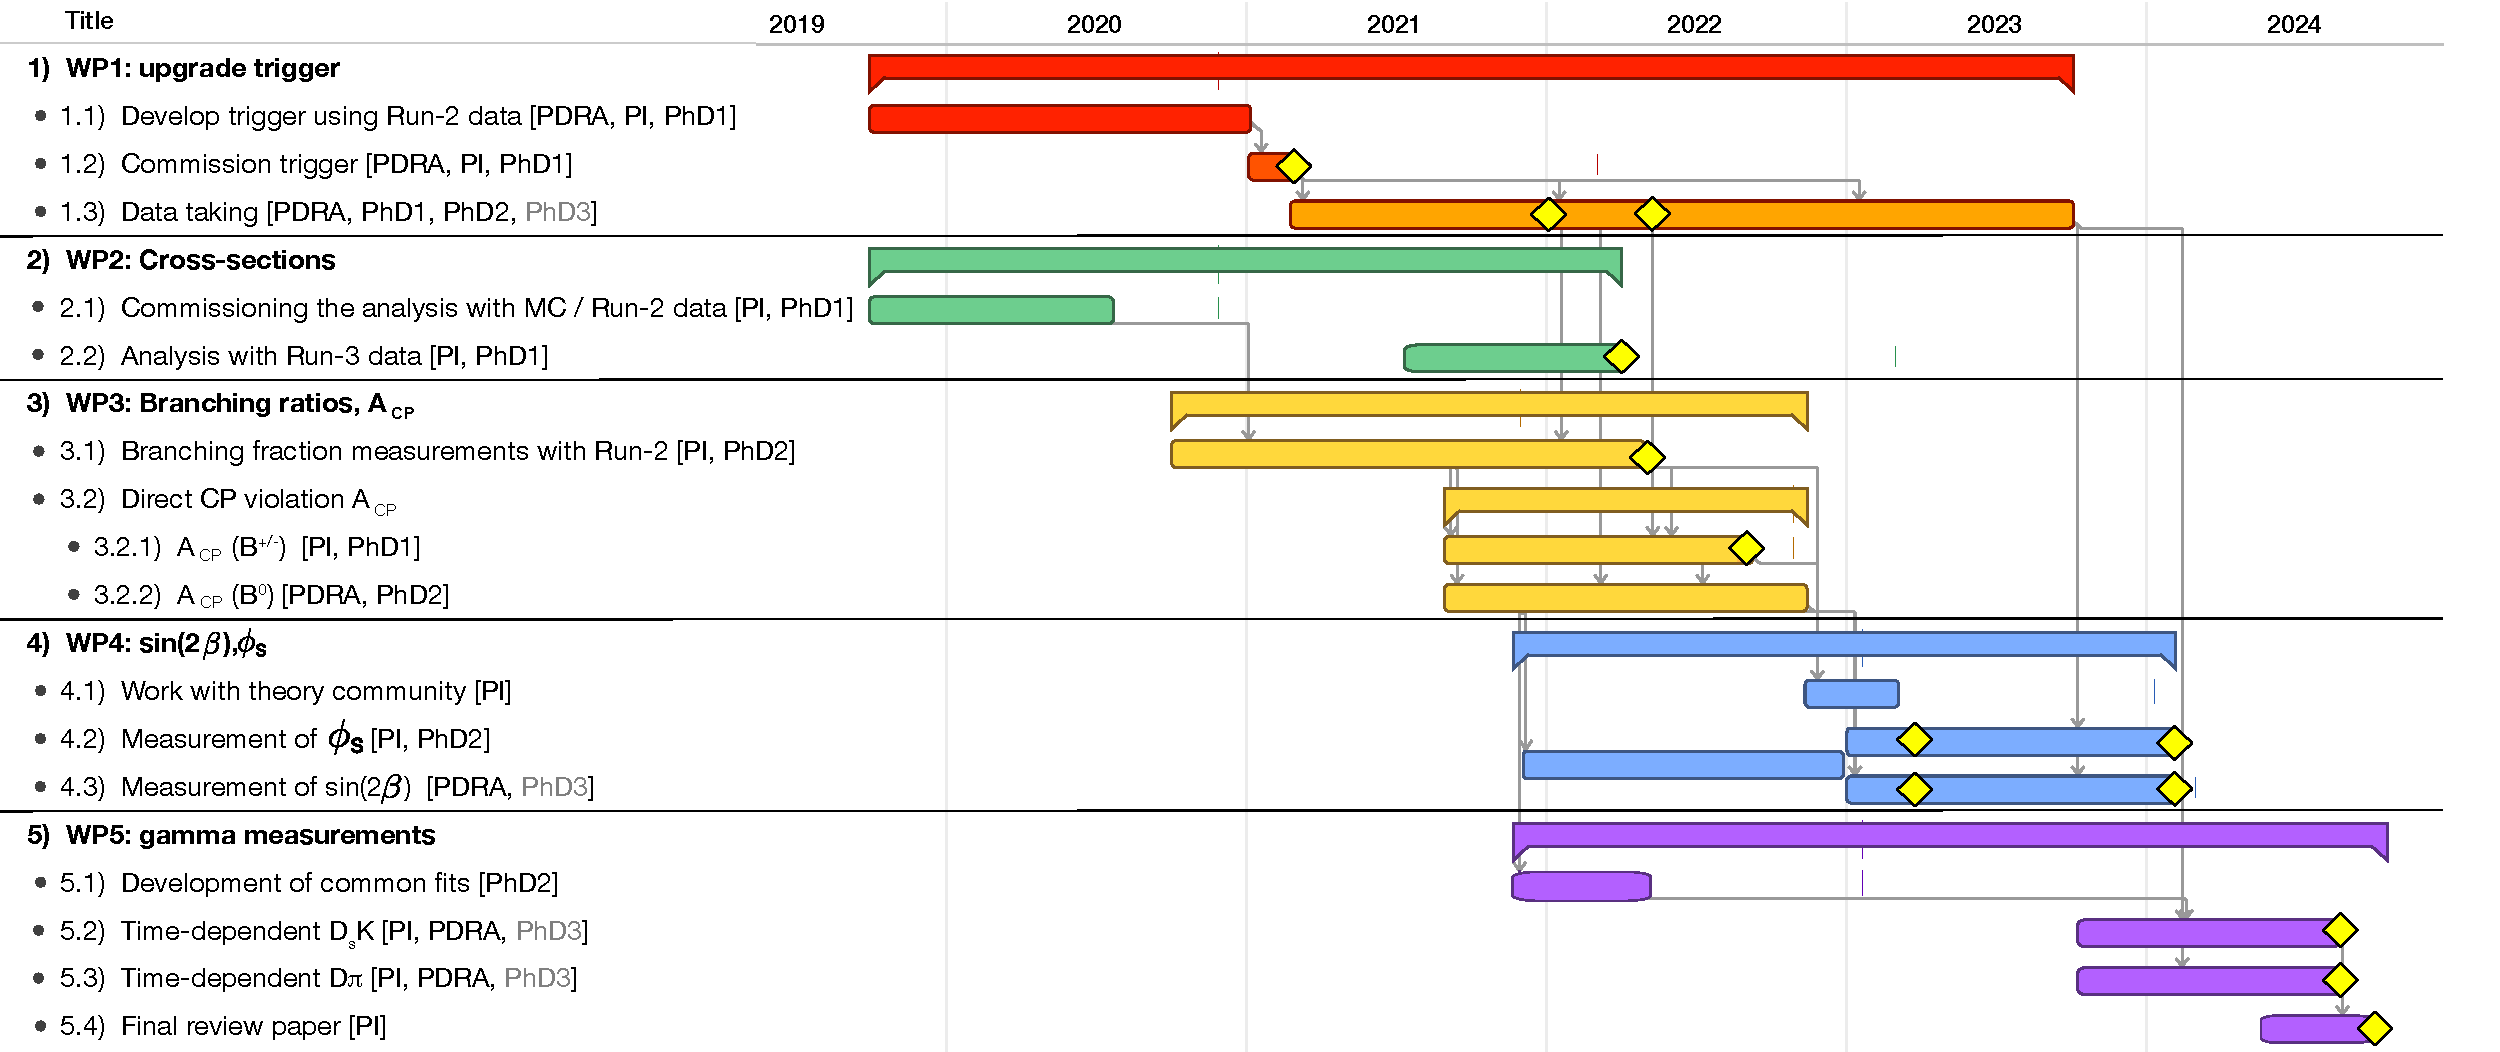
\includegraphics[width=\textwidth]{figs/Gantt_B2_forPublication.pdf}
%\caption{\label{fig:timeline} Detailed project timeline describing the allocation of team members and work %package durations. Vertical lines indicate dependencies between work packages. Publications are marked with %yellow diamonds.}
%\end{center}
%\end{figure}

%The research team will be comprised of the PI, a PDRA, and three PhD students. In the following, a detailed description of the work to be undertaken by the team is given. 

%A timeline describing the overall planning and allocation of team members is provided in Figure~\ref{fig:timeline}. This has been prepared using project planning and management software~\cite{omni:plan}, taking particular care to schedule tasks common to all analyses and balancing the work between the research team in a way that ensures the ambitious project is achievable within the timescale and resources of this research proposal. Resources are discussed in the next section.


\subsection{Risks}
%\smallskip

%\subsubsection{Delays to the LHC and LHCb data taking schedule}
%\subsubsection{Reduced RTA functionality}

\section{Resources}

%The resources requested for this proposal are listed in Table~\ref{tab:resources} and described in detail below. 
%\subsection{Personnel}

%\subsubsection{Principal Investigator} 

%\subsubsection{PDRA}

%\subsubsection{Other personnel}
%Administrative/Clerical support is included at 5\% Full-Time Equivalent (FTE) over the entire five year period. An additional 10\% for computing support is included to maintain the computing cluster and provide technical support related to its use in this project. The Warwick Elementary Particle Physics group is committed to local outreach activities and employs an outreach coordinator. I have an extensive outreach track record and will, along with the PDRA and PhD students participate in local outreach activities. 5\% FTE for outreach support is included. These are costed according to the normal costing procedures at Warwick.

%\subsubsection{Studentships} 
%The proposal seeks funding for two PhD students for 3.5 years each, one to start in year 1 and the second in year 2. A third PhD student, funded by the University of Warwick at no cost to this proposal, will start in year 3. The PhD students will spend their first six months working at 50\% in order to also participate in academic training courses. The last 6 months of the PhD students' time will be spent writing their theses. 

%PhD1 will be hired in the first year, and will initially work with the PI on the WP2 early measurement preparations using the Run 1+2 \LHCb datasets. PhD1 will also participate in development of the RTA reduced event format selections of WP1 with the PDRA. PhD1 is expected to become a trigger and RTA on-call expert based on their experience during the development and commissioning stages, and will be based at CERN on long-term attachment for one year from Q3 2020 to Q3 2021 in order to participate in the early measurement data taking and RTA operations. PhD1 will be an author of the deliverables listed in WP1, the early measurements paper in WP2 and the time-integrated $A_{\text{CP}}$ measurements in WP3.  

%PhD2 will be hired in the second year and will work initially on development of the decay-time-dependent component of the fitting framework in WP3. They will become an expert in flavor tagging calibrations and will be based at CERN on long-term attachment from Q3 2021 to Q3 2023 in order to develop \LHCb-wide flavor tagging procedures as part of the Flavor Tagging Performance working group, in addition to developing the time-dependent fitting framework as part of the Beauty to Open Charm (time-dependent) physics working group. PhD2 will be an author of the Time-dependent measurements in WP3,  and the publications in WP4. They will also contribute to \LHCb-wide flavor tagging performance publications as a result of their work in this proposal.

%\subsection{Travel} 

%\subsubsection{Travel to and from CERN}
%Frequent visits to CERN are required to participate in commissioning, data taking shifts and to disseminate the results of the proposal to the collaboration during \LHCb weeks, when the collaboration meets. Four trips per traveller per year of this kind are envisaged, with 3 travellers in year 1, 4 in years 2
%and 3, 3.5 in year 4 and 2.5 in year 5. 


%\subsubsection{Long-Term Attachment}
%PhD students in high-energy physics are expected, as part of their development, to spend a period of 1-2 years based at their experiment in order to receive training, participate in on-site commissioning and data taking activities and collaborate with their international peer group. Three years of Long-Term Attachment (LTA) at the LHCb experiment at CERN are requested. During this time the students will need to travel to the host institute at the same frequency as described under the previous heading. 

%\subsubsection{Conferences}
%In order to present the results of this proposal to the international community, one conference per person per year is foreseen, with the same number of travellers as listed for CERN visits. 

%\subsection{Equipment}
%The Elementary Particle Physics group has a computing cluster which will be used throughout the course of this project to perform dedicated simulation and pseudoexperiments necessary to determine systematic uncertainties. I have requested funds to add additional processing to the cluster commensurate with the resources the project will require. The costs include additional compute nodes and the warranty required to cover the five year period. 

%\subsection{Other goods and services}
%\subsubsection{Audit}
%The compulsory audit is included at nominal cost. 
%\subsubsection{Recruitment}
%Recruitment costs are included in order to invite prospective PDRA candidates to interview and cover travel expenses. 

%\subsubsection{Training}
%Training is necessary for all members of the proposal in order to aid development and ensure delivery of the proposal objectives. The PDRA and PhD students will take advanced software development courses to aid in the trigger development stage of the project. In addition the PI will take courses in project management and leadership training. 

%\subsubsection{Publication charges}
%The research outputs described in this proposal will be published as a member of the \LHCb collaboration, hosted by CERN. CERN is committed to open access, and covers all publication costs through the SCOAP3 initiative. As such, no publication charges are listed.   

%\subsubsection{Consumables}
%The PDRA and PI will require laptops with an additional screen, and docking station in order to carry out work both in Warwick and when travelling to CERN. Portable backup devices will be purchased for each laptop to mitigate risk of data loss. The laptops will be bought with warranties to cover the duration of the project. These have been included as consumables in Table~\ref{tab:resources}.

\clearpage
\begingroup
    \setboolean{inbibliography}{true}
\bibliographystyle{LHCb}
    \linespread{0.9}\selectfont
\bibliography{researchrefs}

\endgroup


%{\bf Note:} The PI is an author of Refs.~\cite{LHCb-PUB-2014-027,Bourgeois:2018nvk} and all the LHCb collaboration papers, with particular contributions to  Refs.~\cite{Aaij:2014jba,CERN-LHCC-2014-016,Aaij:2013mga,Aaij:2014ywt,LHCb-PUB-2014-040,Aaij:2016kjh,Aaij:2017lff}.
%The PI is acknowledged in Ref.~\cite{Jung:2014jfa}.



\end{document}  
